\documentclass[preprint,3p,review,times,11pt]{elsarticle}

\usepackage{graphicx}
\usepackage{amssymb,amsmath,amsthm}
\usepackage{lineno}
\usepackage{hhline}
\usepackage{fancyhdr,color}
\usepackage{subfigure}
\usepackage{arydshln}		% Tables dash lines, etc
\usepackage{setspace}		% Spacing 
\usepackage{multirow}		
\usepackage{multicol}		% Multicolumns environment
\usepackage[normalem]{ulem}

%%%%%%%%%%%%%%%%%%%%%%%%%%%%%%%%%%%%%%%%%%%%%%%%%%%%%%%%%%%%%%%%%%
\newcommand{\beq}{\begin{equation}}
\newcommand{\eeq}{\end{equation}}
\newcommand{\noin}{\noindent}
\newcommand{\bc}{\begin{center}}
\newcommand{\ec}{\end{center}}
\newcommand{\vc}[1]{\vspace*{#1cm}}
\newcommand{\hc}[1]{\hspace*{#1cm}}
\newcommand{\M}{\mathcal{M}}
\newcommand{\bld}[1]{\boldsymbol{#1}}
\newcommand{\ba}{\bld{a}}
\newcommand{\blc}{\bld{c}}
\newcommand{\bth}{\bld{\theta}}
\newcommand{\bPhi}{\bld{\Phi}}
\newcommand{\bphi}{\bld{\phi}}
\newcommand{\bPsi}{\bld{\Psi}}
\newcommand{\bpsi}{\bld{\psi}}
\newcommand{\bXi}{\bld{\Xi}}
\newcommand{\bxi}{\bld{\xi}}
%%%%%%%%%%%%%%%%%%%%%%%%%%%%%%%%%%%%%%%%%%%%%%%%%%%%%%%%%%%%%%%%%%

%%%%%%%%%%%%%%%%%%%%%%%%%%%%%%%%%%%%%%%%%%%%%%%%%%%%%%%%%%%%%%%%%%

\journal{Computers and Structures}

\begin{document}

\begin{frontmatter}

%% Title, authors and addresses

\begin{center}

\end{center}
\title{Metamodeling of Dynamic Nonlinear Structural Systems through Polynomial Chaos NARX Models}

 \author{M.D. Spiridonakos}
 \author{E.N. Chatzi\corref{cor2}}
 \ead{chatzi@ibk.baug.ethz.ch}
 \cortext[cor2]{Corresponding author, Tel/Fax: (++ 41) 44 633 (direct)}
\address{ETH Zurich, Institute of Structural Engineering,\\
  	Department of Civil, Environmental and Geomatic Engineering, \\ Stefano-Franscini-Platz 5, 8093 Zurich, Switzerland}

\vspace*{-3cm}

\begin{abstract}{
This paper develops a metamodeling methodology that appropriately accounts for uncertainty in the simulation of nonlinear, dynamically evolving engineering systems. Polynomial Chaos (PC) expansion offers a useful tool for the development of stochastic metamodels capable of representing the random response of analytical/numerical models with uncertain input variables. This approach relies upon the approximation of the random response of an analytical model by a suitably defined finite-dimensional PC basis in order to create a low order metamodel. The latter is considered to be of the Nonlinear AutoRegressive with eXogenous input (NARX) model form with parameters that are random variables themselves. By expanding these parameters onto an appropriately selected PC basis the resulting PC-NARX metamodel is fully described by a finite number of deterministic coefficients of projection which may be estimated by linear or nonlinear regression. In order to illustrate the workings of the method, the whole procedure is applied for the construction of metamodel representations of both simple analytical nonlinear models, namely a system with nonlinear elasticity, a hysteretic system, and a five-storey shear frame numerical model relating to a common structural system of multiple degrees of freedom. Overall, this study aims at demonstrating the effectiveness and applicability of the proposed method for the estimation of stochastic metamodels of low order that are capable of accurately approximating of nonlinear structural models. }
\end{abstract}

\vspace*{1cm}

\begin{keyword}
Metamodels \sep Polynomial chaos expansion\sep NARX modeling \sep Finite element models\sep dynamic responses\sep structures.
\end{keyword}

\end{frontmatter}
 

% ===============================================
\section{Introduction}
% ===============================================
Numerical modeling has long been the main tool for the handling of complex engineering problems. The development of the Finite Element (FE) method, starting with the seminal contributions of Argyris and Kelsey \cite{Argyris-Kelsey1955} and Turner et al. \cite{Turner-etal1956} and further established by R. Clough \cite{Clough1960} in the 1960s offered a strong tool for the computational modeling of large engineering systems. The method has since been extensively used in a number of civil, mechanical, aeronautical and electrical engineering applications \cite{Bathe2009}. In the more recent years, especially in the field of Structural Health Monitoring (SHM) which has come to be a significant branch of civil engineering research, detailed FE models have been utilized for various ends including design optimization \cite{Chang-Perl1988}, inverse problem formulation for damage detection \cite{Waisman-etal2010, Rabinovich-etal2007}, structural model updating \cite{Papadimitriou-etal2012, Mottershead-Friswell1993}, and assessment of the dynamic response of a structural system especially for the case of nonlinear behavior usually related to hysteresis \cite{Taucer-etal1991, Triantafyllou-Koumousis2012}. For reasons of safety, the latter issue is particularly important for civil structures, such as buildings and bridges, subjected to extreme loading conditions like earthquakes and strong winds which cause the structure to shift  outside the usual assumption of linear response.


The advancements achieved in the field of Finite Element (FE) modeling methods have played a key role in overcoming this hurdle by enabling the realization of sophisticated simulation experiments emulating structural response \cite{Bathe2009}. However, despite the rapidly growing computational power and the continuous development of increasingly efficient algorithms, the also growing complexity of FE models and the necessity for more detailed descriptions of both structural geometry and mechanical properties renders the use of highly detailed FE models almost prohibitive for complex, large structures \cite{Gholizadeh-Salajegheh2009}. In order to treat this problem, it is a common task in structural analysis to use less refined macro-model systems for the simulation of global behavior and more detailed local FE models for the simulation of complex parts of the structure (i.e. joints, connections and so on). 

Nevertheless, the problem is even more pronounced when taking into account that the structural systems are commonly characterized by parameter uncertainty to what concerns for instance the mechanical properties of the structure. Thus, the analyst is faced with the task of performing a number of simulations in order to obtain an accurate numerical model of an existing structure. Moreover, when the linearity assumption is relaxed in favor of increased modeling accuracy the numerical model must be tested for a number of different excitation scenarios. Thus, for the extensive experimentation required for design optimization or model updating procedures based on time history loading, a simpler representation of the FE model should be considered which should also be able to describe the behavior of the structure for a wide range of excitations.  In such cases, traditional approaches like the Monte Carlo methods, which usually necessitate a large number of simulations cannot be used, since the simulations themselves are associated with excessive computational cost. 

For the extensive experimentation required for design optimization or model updating procedures based on time history loading and on-line response measurements, a simpler representation of the numerical model should be considered. Different approaches have been investigated for the reduced order modeling of complex engineering systems with the resulting representation, which actually constitutes a model of a model, usually termed as metamodel or surrogate model \cite{Yesilyurta-Patera1995}. This metamodel must be able to predict the detailed numerical model dynamic response in a computationally inexpensive way and with sufficient accuracy. In this way, once an early prediction is achieved through the use of the metamodel, a more refined analysis can then take place using the full scale FE model in the identified area of interest. The Proper Orthogonal Decomposition (POD) methods \cite{Du-Gunzburger2002} and reduced-basis methods \cite{Peterson1989} have been formulated within such a context for fluid dynamics problems, while the Gyan condensation method and the System Equivalent Reduction Expansion Process \cite{Papadopoulos-Garcia1996} have also been used for the reduction of structural models. 


The main goal of the present study is the development of a metamodeling method which should be able to provide reduced representations of large numerical systems for the accurate simulation and/or prediction of their dynamic response. The motivation comes from the common issue of attempting to simulate intricate structural systems subjected to dynamic loading, a process which is known to require high computational resources. This is an important task especially for the case of inverse problem formulations where the goal is to accurately represent experimentally measured behavior \cite{Fuggini-etal2011}. The metamodeling method introduced herein is based on models of the Nonlinear AutoRegressive with eXogenous input (NARX) form, with random parameters utilized for the description of uncertainty propagation through the numerical model. The random NARX model parameters are expanded onto a Polynomial Chaos (PC) basis and thus the resulting PC-NARX model is fully described through deterministic coefficients of projection estimated through least squares optimization. The PC method has recently been intensively examined for the evolution of uncertainty in dynamical systems, in the presence of probabilistic uncertainty in the system parameters \cite{Li-Ghanem1998, Sapsis-Lermusiaux2012, Gerritsma-etal2012}.

In order to illustrate the proposed method's efficiency, and following two numerical examples based on simple single degree of freedom nonlinear systems, the PC-NARX modeling procedure is applied for the construction of a metamodel of a shear frame model which is subjected to dynamic excitation leading to nonlinear response. The Young modulus of the model elements is assumed to be uncertain following a prescribed probability distribution, while the metamodel is estimated from simulated data obtained by the FE model for a relatively small number of experiments.  

The paper is organized as follows: The description of the PC-NARX class of models is given in Section \ref{sec:PCNARX} along with the proposed model parameter and model structure selection methods which are presented in Sections \ref{sec:MPE} and \ref{sec:MSS}, respectively. The numerical application involving the simple SDOF systems and the shear frame FE model, the conducted simulations and the metamodeling results are presented in Section \ref{sec:numerical}, while the main conclusions of the study are drawn in Section \ref{sec:conclusions}.


% ===============================================
\section{POLYNOMIAL CHAOS NARX METAMODELS}
% ===============================================
\label{sec:PCNARX}

Let us consider a structural system represented by a numerical model $\mathcal M$ that is characterized by a number of input variables related with the properties of the modeled structure (mechanical and/or geometric). It is assumed that $M_1$ of these parameters are subject to uncertainty and that they may be described by independent random variables gathered in a random vector $\bxi_S = [ \xi_{1}, \xi_{2},\ldots ,\xi_{M_1} ]^T$. Superscript $T$ denotes transpose of a vector or a matrix while it is noted that for simplicity of notation no distinction is made between a random variable and its value(s).

Since the dynamic behavior of a nonlinear numerical model is also a function of the input excitation characteristics, it is considered that the set of excitation signals used for the dynamic loading of the numerical model may be described by a small number of random variables $\bxi_X = [ \xi_{M_1+1}, \xi_{M_1+2},\ldots ,\xi_{M_1+M_2} ]^T$. 

As a result of the uncertainty propagation, the dynamic response of the numerical model to a given input excitation will also be a random variable which in addition depends on time, that is
%%
\beq 
y[t,\bxi] = {\mathcal M}(x[1,\bxi_X],x[2,\bxi_X],\ldots,x[t,\bxi_X],\bxi_S)
\eeq
%%
with $t = 1,2,\ldots, N $ designating normalized by the sampling period discrete time, $x[t,\bxi_X]$ the excitation input signal, $y[t,\bxi]$ the corresponding numerical model response signal, and $\bxi = [ \bxi_S^{T} \ ,\ \bxi_X^{T} ]^{T}$ the $M$-dimensional ($M = M_1 + M_2$) complete vector of input random variables with known joint probability density function (pdf) $f(\bxi)$ . 


Metamodeling refers to the process of identifying a reduced order and computational complexity representation $\widetilde{\mathcal M}$ of the large scale numerical model ${\mathcal M}$. In the present work, a metamodel is sought for the accurate representation of the dynamics of the numerical model and the accurate simulation and/or prediction of its time history loading response $y[t,\bxi]$. 

In order to approximate the numerical model dynamic response $y[t,\bxi]$ for every realization of $\bxi$ in an efficient way, a novel metamodeling method based on Polynomial Chaos Nonlinear AutoRegressive with eXogenous input (PC-NARX) models is introduced. The general PC-NARX model, in the linear-in-the-parameters form, is given by the following relationship \cite{Chen-Billings1989}:
%%
\beq \tilde{y}[t,\bxi] =  \sum_{i=1}^{n_\vartheta} \vartheta_i(\bxi) \cdot g_i({\bld z}[t,\bxi]) + e[t] \label{eq:PCNARX}\eeq
%%
where $n_\vartheta$ is the number of nonlinear model terms $g_i({\bld z}[t,\bxi])$ that are generated from the regression vector ${\bld z}[t,\bxi] = \left\{ \tilde{y}[t-1,\bxi], \ldots, \tilde{y}[t-n_a,\bxi],  x[t,\bxi_X],\ldots ,x[t-n_b,\bxi_X] \right\}^T$ with $n_a, n_b$ designating the maximum output and input time lags, respectively, and $e[t]\! \sim\! \text{NID} (0,\sigma^2_e)$ the model's residual sequence with NID$(\cdot,\cdot)$ denoting normally independently distributed process with the indicated mean and variance. It should be mentioned that the model terms $g_i({\bld z}[t,\bxi])$ may be constructed from a variety of local or global basis functions including polynomials, splines, neural networks, wavelets and others \cite{Wei-Billings2009}.

The important feature of PC-NARX models, in comparison with the conventional NARX models \cite{Chen-Billings1989}, is that they are characterized by parameters $\vartheta_i(\bxi)$ which are random variables themselves. The latter are actually represented by a deterministic mapping which which describes their relationship to the input random variables. More specifically, assuming that the PC-NARX model parameters $\theta_i(\bxi)$ have finite variance, they admit the following polynomial chaos representation \cite{Soize-Ghanem2004}:
%%
\beq 
\vartheta_i (\bxi) = \sum_{j=1}^{\infty } \theta_{i,j}\cdot \phi_{\bld{d}(j)}(\bxi) \label{eq:PCE}
\eeq
%%
where $\theta_{i,j}$ are unknown deterministic coefficients of projection, ${\bld d}{(j)}$ is the multi-indices of the multivariate polynomial basis, and $\phi_{{\bld d}(j)}$ are multivariate basis functions that are orthonormal with respect to the joint pdf of $\bxi$, that is:
%%
\beq
E[ \phi_{\bld \alpha} (\bxi), \phi_{\bld \beta} (\bxi) ] = \delta_{{\bld \alpha},{\bld \beta}} =\begin{cases} 1 & \mbox{for } \alpha = \beta \\ 0 & \mbox{otherwise} \end{cases}
\eeq
%%
Each probability density function may be associated with a well known family of orthogonal polynomials. For instance, the normal distribution is associated with Hermite polynomials while the uniform distribution with Legendre. A list of the most common probability density functions along with the corresponding orthogonal polynomials and the formulas for their derivation may be found in \cite{Soize-Ghanem2004}.

For purposes of practicality, the basis functions series must be truncated to a finite number of terms, with the usual approach being the selection of the multivariate polynomial basis with total maximum degree $| {\bld d}(j)| = \sum_{m=1}^{M} d{(j,m)} \leq P $ for every $j$. In this case, the dimensionality of the functional subspace is equal to
%%
$$ p = \frac{(M+P) !}{M! P !}$$
%%
where $M$ is the number of random variables and $P$ the maximum basis degree. For instance, for a random input vector of dimension equal to three ($M=3$) and maximum degree equal to two ($P = 2$) the multi-indices vectors are:
%%
$$
\begin{array}{r | cccccccccc}
& {\bld d}{(1)} & {\bld d}{(2)} & {\bld d}{(3)} & {\bld d}{(4)} &
{\bld d}{(5)} & {\bld d}{(6)} & {\bld d}{(7)} & {\bld d}{(8)} &  
{\bld d}{(9)} & {\bld d}{(10)} \\ \hline
{\bld 1} & 0 & 1 & 0 & 0 & 1 & 1 & 0 & 2 & 0 & 0 \\
m \quad {\bld 2} & 0 & 0 & 1 & 0 & 1 & 0 & 1 & 0 & 2 & 0 \\
{\bld 3} & 0 & 0 & 0 & 1 & 0 & 1 & 1 & 0 & 0 & 2 \\
\end{array}
$$
%%
Therefore, truncating the infinite series of expansion of Eq. (\ref{eq:PCE}) to the first $p$ terms the resulting PC-NARX model is fully parametrized in terms of a finite number of deterministic coefficients of projection $\theta_{i,j}$ while a specific PC-NARX model structure is fully defined by the nonlinear regressors, and the polynomial degree $P$. 


The complete PC-NARX identification problem may thus be stated as follows: Given a set of excitation signals and the corresponding dynamic response signals obtained from the numerical model under study for different input parameter vector realizations, select the PC-NARX model structure and the corresponding model parameters that best fit the available records. The issues of PC-NARX model parameter estimation and model structure selection are discussed in the following sections. 


% =================================================================================================
%% IMPROVE 
% =================================================================================================

At this point it should be noted that PC-ARIMA models with a-priori known deterministic coefficients of projection have been considered in the literature for the characterization of terrain topology by Wagner and Ferris \cite{Wagner-Ferris2007}. Moreover, linear PC-ARX models have used in the metamodeling context in \cite{Spiridonakos-Chatzi2012}. Similarly linear ARX models with functionally dependent parameters have also been used in a number of studies for the purposes of structural identification and damage detection (for instance see \cite{Kopsaftopoulos-Fassois2012} and the references therein). However, the aforementioned methods are not suitable for describing nonlinearities which have the additional issue of input dependence, while also input variables are not related to a known probability density function and thus the basis is constructed from an arbitrarily selected family of orthogonal basis functions. 
% =================================================================================================


%=========================================================================
\subsection{Parameter estimation}\label{sec:MPE}
%=========================================================================

As already mentioned, the estimation of a PC-NARX metamodel refers to the determination of the coefficients of projection parameter vector $\bth$ 
%%
\beq \bth = [\, \theta_{1,1} , \, \theta_{1,2}, \, \ldots ,\, \theta_{n_\vartheta,p} \, ]^T \eeq 
%%
or a subset of $\bth$ selected by the procedure described in the following section. The estimation is based on the availability of time history data for the input excitation and output response of the numerical model. These may be acquired for a series of simulations, conducted for different realizations of the input random vector using the full scale numerical model.


It is considered that a series of $K$ simulations conducted for a corresponding number of input random vector realizations $\bxi_k = [\xi_{k,1}, \xi_{k,2}, \ldots ,\xi_{k,M}]^T$ (with $k=1,2,\ldots,K$), and the resulting set of excitation signals ${\bld x}_k^N = \{ x_k[1], x_k[2], \ldots, x_k[N] \}$ are available. It is noted that for the purposes of notational simplicity the dependency of the input and output signals on $\bxi_k$ is not indicated explicitly in the following relationships.

The corresponding dynamic response of the full scale numerical model is indicated as ${\bld y}_k^N = \{ y_k[1], y_k[2],$ $\ldots, y_k[N] \}$ and as already mentioned it is assumed to follow the general PC-NARX model of equation (\ref{eq:PCNARX}):
%%
\begin{subequations} \label{eq:assumptions}
\begin{align} & y_k[t] = \sum_{i=1}^{n_\vartheta} \vartheta_i(\bxi_k) \cdot g_i(z_k[t]) + e_k[t], \label{eq:exp_n} \\  
& e_k[t] \sim  \mbox{NID}(0,\sigma_{e_k}), \\ 
& E\{ e_i [t], e_j[ t - \tau ] \} =  
\begin{cases} 
\sigma^2_{e_i} \cdot \delta_{t,\tau} & \mbox{ for } i = j \\
 0 &  \mbox{ for } i \neq j \end{cases}
\end{align}
\end{subequations}
%%
In the relationships above, the uncorrelatedness of the residual series between different simulation experiments is also assumed. For these simulations, the input vector $\bxi_k$ is generated from the input parameter space either randomly or by using a structured sampling technique, such as the Latin Hypercube Sampling (LHS; \cite{Helton-Davis2003}).

As already mentioned, a metamodel that may replace the numerical model for additional simulations is sought. Toward this end, the estimation of the parameter vector $\bth$ may be based upon the minimization the Simulation Error (SE) criterion. 


% ===============================================
\subsubsection{Simulation error method} \label{sec:SEestimation}
% ===============================================
Let us consider again the same set of $K$ input excitation signals ${\bld x}_k^N (k = 1, 2, \ldots,K)$. For each ${\bld x}_k^N$ the simulated response $\tilde{\bld y}_k^N$ of a PC-NARX metamodel may be obtained by using the input excitation signals and the following relationship applied recursively with respect to time $t$:
%%
\beq 
\tilde{y}_k[t] = \sum_{i=1}^{n_\vartheta} \vartheta_i (\bxi_k) \cdot g_i(\tilde{\bld z_k}[t]) = \sum_{i=1}^{n_\vartheta}\sum_{j=1}^{p}  \theta_{i,j} \cdot \phi_{\bld{d}(j)}(\bxi_k) \cdot g_i(\tilde{\bld z}_k[t]) \label{eq:ysim}
\eeq
%%
with given initial conditions $\{ y_k[1 - n_a], \ldots, y_k[0] \}$ and $\{ x_k[1-n_b,\bxi_X], \ldots, x_k[0,\bxi_X]\}$. The responses $\tilde{y}_k[t]$ of the metamodel should be as close as possible to that of the numerical model $y_k[t]$, thus the estimation of a PC-NARX metamodel may be based on the minimization of the following SE criterion: 
%%%
\begin{align} \label{eq:SIMcrit} \hat{\bth} & = \arg\min_{\bth_s} \left\{ \sum_{k=1}^K \sum_{t=1}^N  (y_k[t]- \tilde{y}_k[t] )^2 \right\} \nonumber \\
&= \arg\min_{\bth_s} \left\{ \sum_{k=1}^K \sum_{t=1}^N  \varepsilon_k^2[t] \right\}
\end{align}
%%%
This optimization problem may be solved by iterative nonlinear optimization methods. However, these methods are typically amenable to wrong convergence problems when initialized by arbitrary or inaccurate estimates. For this reason, the SE method may be initialized by the parameter vector $\bth$ obtained through the PE method described in the following section.

% ===============================================
\subsubsection{Prediction error method} \label{sec:PEestimation}
% ===============================================
The PE criterion consists of the sum of squares of the model's one-step-ahead prediction errors for the complete set of simulation experiments. As it may be easily shown the one-step-ahead prediction errors coincide with the model's residual sequence and thus $\bth$ has to be estimated by the following minimization problem:
%%
\begin{eqnarray} 
\hat{\bth} & = & \arg\min_{\bth} \biggl\{ \sum_{k=1}^K \sum_{t=1}^N  (y_k[t] - \hat{y}_k[t|t-1])^2 \biggr\} \nonumber\\ 
& = & \arg\min_{\bth} \biggl\{ \sum_{k=1}^K \sum_{t=1}^N  e_k^2[t] \biggr\} \label{eq:PEcrit} 
\end{eqnarray}
%% WLS criterion
%\begin{eqnarray} 
%\hat{\bth} & = & \arg\min_{\bth} \biggl\{ \sum_{k=1}^K \sum_{t=1}^N  \frac{(y_k[t] - \hat{y}_k[t|t-1])^2}{\gamma^2_k} \biggr\} \nonumber\\ 
%& = & \arg\min_{\bth} \biggl\{ \sum_{k=1}^K \sum_{t=1}^N  \frac{ e_k^2[t]}{\gamma^2_k} \biggr\} \label{eq:PEcrit} 
%\end{eqnarray}
%%
%with $ \hat{y}_k[t|t-1]$ designating the model's one-step-ahead prediction, $\gamma_k$ user defined weights, and $\arg\min$ minimizing argument. Toward this end, and by using Eq. (\ref{eq:PCE}), Eq. (\ref{eq:exp_n}) may be rewritten as:
%%
with $ \hat{y}_k[t|t-1]$ designating the model's one-step-ahead prediction and $\arg\min$ minimizing argument. Toward this end, and by using Eq. (\ref{eq:PCE}), Eq. (\ref{eq:exp_n}) may be rewritten as:
%
$$ y_k[t]  =  \sum_{i=1}^{n_\vartheta}\sum_{j=1}^{p}  \theta_{i,j} \cdot \phi_{\bld{d}(j)}(\bxi_k) \cdot g_i(\bld{z}_k[t]) + e_k[t] \Rightarrow $$
\beq y_k[t]  = {\underbrace{\left[\begin{array}{c}
\phi_{\bld{d}(1)}(\bxi_k) g_1(\bld{z}_k[t]) \\
\vdots\\
\phi_{\bld{d}(p)}(\bxi_k) g_{n_\vartheta}(\bld{z}_k[t]) \\
\end{array}\right]}_{\bphi [\bxi_k,t]}}^{T}   \cdot  \left[  \begin{array}{c}
\theta_{1,1} \\
\vdots\\
\theta_{n_\vartheta,p} \\
\end{array} \right] +  e_k[t]
\eeq
%%
or by stacking all time-instants in a single vector
%
$$ 
\underbrace{\left[\begin{array}{c}
y_k[1] \\
y_k[2] \\
\vdots\\
y_k[N] \\
\end{array}\right]}_{\bld{y}_{k_{[N \times 1]}}} = \underbrace{\left[\begin{array}{c}
\bphi [\bxi_k , 1]^{T}  \\
\bphi [\bxi_k , 2]^{T}  \\
\vdots \\
\bphi [\bxi_k , N]^{T}  \\
\end{array}\right]}_{\bPhi(\bxi_k)_{[N \times  n_\vartheta p ]}} \cdot \underbrace{\left[\begin{array}{c}
\theta_{1,1} \\
\vdots\\
\theta_{n_\vartheta,p} \\
\end{array}\right]}_{\bth_{[ n_\vartheta p \times 1]}} + \underbrace{\left[\begin{array}{c}
e_k[1] \\
e_k[2] \\
\vdots\\
e_k[N] \\
\end{array}\right]}_{\bld{e}_{k_{[N \times 1]}}}
$$
%%
where subscripts in brackets indicate the respective matrix/vector dimensions. Finally, by pooling all the available simulation experiments, the following linear regression model is obtained:
\beq 
\label{eq:regression}
\underbrace{\left[\begin{array}{c}
\bld{y}_1^N \\
\bld{y}_2^N \\
\vdots\\
\bld{y}_K^N \\
\end{array}\right]}_{\bld{Y}_{[K N \times 1]}} = \underbrace{\left[\begin{array}{c}
\bPhi(\bxi_1)\\
\bPhi(\bxi_2)\\
\vdots \\
\bPhi(\bxi_K)
\\
\end{array}\right]}_{\bPhi(\bxi)_{[K N \times n_\vartheta p ]}} \cdot \underbrace{\left[\begin{array}{c}
\theta_{1,1} \\
\vdots\\
\theta_{n_\vartheta,p} \\
\end{array}\right]}_{\bth{[ n_\vartheta p \times 1]}} + \underbrace{\left[\begin{array}{c}
\bld{e}_1^N \\
\bld{e}_2^N \\
\vdots\\
\bld{e}_K^N \\
\end{array}\right]}_{\bld{E}_{[K N \times 1]}}
\eeq
%%
where $\bPhi(\bxi)$ is the regression matrix. Thus, the minimization problem of equation (\ref{eq:PEcrit}) may be rewritten as follows:
%%
% \beq \hat{\bth} =\arg\min_{\bth} \left\{ {\bld E}^{T} \cdot {\bld \Gamma} \cdot {\bld E} \right\}\eeq
\beq \hat{\bth} =\arg\min_{\bth} \left\{ {\bld E}^{T} \cdot {\bld E} \right\}\eeq
%%
% where ${\bld \Gamma} = {\bld I}_N \otimes {\bld \gamma} $ with ${\bld \gamma} = [\gamma_1,\ldots, \gamma_K]^T$ denoting the vector of weights, ${\bld I}_N$ the $N\times N$ identity matrix, and $\otimes$ the Kronecker product operator.
% Due to the linear dependence of the residual sequence ${\bld E}$ on the parameter vector ${\bth}$ the last equation leads to a linear weighted least squares estimator for the latter, that is: 
which due to the linear dependence of the residual sequence ${\bld E}$ on the parameter vector ${\bth}$ the last equation leads to a linear least squares estimator for the latter, that is: 
%%
\beq
% \hat{\bth} = \bigl(\bPhi^{T}(\bxi) \cdot {\bld \Gamma} \cdot \bPhi(\bxi) \bigr)^{-1} \cdot \bigl( \bPhi(\bxi)^{T} \cdot {\bld \Gamma} \cdot {\bld Y} \bigr)  
\hat{\bth} = \bigl(\bPhi^{T}(\bxi) \cdot \bPhi(\bxi) \bigr)^{-1} \cdot \bigl( \bPhi(\bxi)^{T} \cdot {\bld Y} \bigr)  
\eeq

% The simplest and obvious choice for the weights $w_k$ is to set them equal to unity, with this selection leading to the ordinary least squares estimator. However, it has been shown for the, also linear-in-the-parameters, FP-ARX models \cite{Kopsaftopoulos-Fassois2012} that the weights that lead to consistent and asymptotically efficient estimates are equal to the standard deviation of the residual sequence, that is
%%
% \beq
% \gamma_k^2 = \sigma_{{\bld e}_k}^2, \quad \text{for } k = 1,\ldots,K
% \eeq
%%   
% However, the true residual variance is a priori unknown and has to be replaced by an appropriate estimate, which is normally obtained by the OLS estimation utilized as a first stage. The WLS estimator may then be realized in an iterative way till convergence that may be defined in terms of either the PE criterion or the coefficients of projection estimates $\hat{\bth}$. 

It should be noted that, beyond their use as initial estimates for the SE method, PC-NARX models estimated through the PE method may also be used for on-line prediction of the dynamic response, when the structural system corresponding to the numerical model is appropriately instrumented. This metamodel may in turn be used for a number of purposes such as vibration control, structural health monitoring, model updating and others. Typically this process is especially helpful for problems where direct feedback of response is required.


%================================================
\subsection{Model structure selection}\label{sec:MSS}
%================================================

Model structure selection may be considered as the optimization procedure during which models corresponding to various candidate ``structures'' are estimated (through the methods of the previous section), and the one providing the {\em ``best fitness''} to the simulation data is selected.

The specific family of nonlinear functions (e.g. polynomials, splines, neural networks, or wavelets), the maximum output and input lags $n_a$ and $n_b$ may be chosen based on known structural properties of the numerical model to be approximated, such as the number of degrees of freedom and the type of nonlinearlity that exhibits. However, the number of candidate regressors is usually large even after a mindful choice. Thus, the selection of only a small number of adequate regressors may not be based on a trial-and-error approach. Moreover, the estimation of a single PC-NARX model based on SE estimation is computationally demanding even for moderate model sizes. 

In order to overcome these issues a two-phase PC-NARX model structure selection procedure is presently proposed. These phases concern the determination of: \emph{i)} the nonlinear model terms $g_i({\bld z}[t])$ and \emph{ii)} the PC basis functional subspace, while they are performed at low computational cost.

%================================================
\paragraph{\bf \em Local-NARX models estimation}
%================================================
The first phase deals with the selection of the appropriate nonlinear terms $g_i({\bld z}[t,\bxi])$ and the estimation of local-NARX models for each one of the data sets $\{ {\bld x}_k^N , {\bld y}_k^N \} (\text{for } k = 1,\ldots, K)$. Towards this end, the selection of the nonlinear model terms is based on the NARX modeling of the dataset exhibiting the highest nonlinearity, assuming that this set will require the maximum number of nonlinear terms for its accurate representation. This dataset may be chosen either based on nonlinearity quantification criteria \cite{Choudhury-etal2008}, or by inspection of the set of the uncertain parameters responsible for the onset of nonlinearity. 

Assuming that simulation experiment $k_o$ is selected for this purpose, the excitation signal $\bld{x}_{k_o}^N$ and the simulated response $\bld{y}_{k_o}^N$  are going to be used for this purpose while the initial search space has been predefined (e.g. $\{ y[t-1], y[t-1]^2 , y[t-1]^3, x[t],x[t]^2,x[t]^3 \}$). Initially, Genetic Algorithm (GA) optmization is used in order to determine promising subregions of the complete search space. Each candidate model created by the GA, is estimated by means of the PE method, though is judged in terms of its simulation capabilities. This simplification is based on an implicit assumption on the proximity of the PE-based and SE-based estimated models and is employed in order to circumvent the nonlinear optimization required for each individual within the GA optimization procedure. 

Each GA individual is a bit-string, with each bit representing the existence (1) or not (0) of the corresponding nonlinear term from the initial search space. For example considering the initial search space given in the previous paragraph, each individual will be represented by a 6-bit vector, with an hypothetical optimal solution $[1 0 1 1 0 0]$ corresponding to ${\bld g}({\bld z}[t]) = \{ y[t-1], y[t-1]^3, x[t] \}$.          

In order to refine and potentially reduce model dimensionality, the concept of backward regression may be used as a second step. Starting from the GA solution, the nonlinear term whose removal has the minimum effect on the SE criterion is dropped, with the procedure being repeated till no more regressors are available. In this way, only the nonlinear terms which have a significant effect on the SE criterion are retained. 

This phase is completed by estimating a local NARX model with the selected structure for each simulation experiment. For this phase, SE nonlinear optimization initialized by PE-based estimates is performed. 


%% ==============================================
\paragraph{\bf \em PC subspace selection}
%% ==============================================

This second phase, is based on the estimated parameters $\hat{\vartheta_i} (\bxi_k)$'s of the local NARX models and GA in order to define appropriate PC subspaces for their expansion, providing at the same time initial estimates for the PC-NARX coefficients of projection $\theta_{i,j}$.   

Toward this end, Eq. (\ref{eq:PCE}) is utilized for expanding the parameters $\hat{\vartheta_i} (\bxi_k)\ (i = 1,\ldots, n_\vartheta \text{ and } k = 1,\ldots, K)$, which are treated as measurements, onto candidate PC subspaces by using least squares optimization. The initial search space is defined by the complete PC basis with maximum total degree equal to $P$ while each individual is again represented as a binary vector, with each bit denoted the inclusion (1) or not (0) of a specific multivariate basis function into the candidate subspace. The maximization criterion used, is the mean value of the adjusted $R^2$ values \citep{Blatman-Sudret2010}, that is: 
%
\beq 
\overline{R^2_\text{adj}} = \frac{1}{n_\vartheta} \sum_{i=1}^{n_\vartheta} R^2_{\text{adj}_i}, \text{ where } R^2_{\text{adj}_i} = 1 - \frac{ \sum_{k=1}^K \left( \hat{\vartheta_{i}}(\bxi_k)  - \sum_{j=1}^{p} \theta_{i,j}\cdot \phi_{\bld{d}(j)}(\bxi_k) \right)^2} {\sum_{k=1}^K \left(\hat{\vartheta_{i}}(\bxi_k) - \overline{\hat{\vartheta}(\bxi_k)}\right)^2}  \cdot \frac{K-1}{K-p-1}\label{eq:PCEerror}
\eeq
%
which includes a penalty term for the dimension of the expansion space. In the equation above, overline denotes mean value of the indicated quantity.       


Then, the selected PC subspace may be further reduced by dropping one by one the bases till all of them are dropped. The bases are dropped by using again the criterion of Eq. (\ref{eq:PCEerror}), with the bases whose removal leads to a significant decrease of $\overline{R^2_\text{adj}}$ being finally retained. 





% ================================================
\section{Numerical examples}\label{sec:numerical}
% ================================================


% ================================================
\subsection{Nonlinear single degree of freedom systems}
% ================================================

The test cases of two SDOF nonlinear oscillators are presently examined. The SDOF oscillators are mass-damper systems with an additional element producing a nonlinear restoring force $F(t)$ (Fig. \ref{fig:SDOF}):
%
\beq m \ddot{y}(t) + c\dot{y}(t) + F(t) = x(t) \label{eq:SDOF}\eeq
%
In the first example the restoring force is due to a nonlinear (cubic) in parallel with a linear spring, while in the second case the restoring force is due to a hysteretic system described by a simplified Bouc-Wen model. The purpose of choosing these particular systems lies in the nature of these two test cases. In the first case polynomial NARX regressors are able to fully describe the dynamics of the system while in the second case the form of the NARX regressors is more complex.


% Figure
% ================================================
\begin{figure}[t]
\centering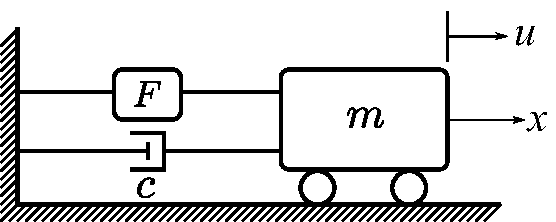
\includegraphics[width = 0.5\textwidth]{figs/SDOF.pdf}
\caption{Single degree of freedom system with nonlinear restoring force.}\label{fig:SDOF}
\end{figure}
% ================================================



% ================================================
\subsubsection{Cubic stiffness}
% ================================================

In this first paradigm the restoring force is due to the placement of a linear and a cubic stiffness spring in parallel and thus described by the following equation: 
%
\beq F(t) = k{y}(t) + k_{\mathrm{nl}}{y}(t)^3  \label{eq:cubic_restoring}\eeq
%
The nonlinear SDOF system is considered to be subject to stationary random force with uncertain standard deviation while it is also characterized by uncertainty of the cubic stiffness coefficient $k_{\mathrm{nl}}$. The properties of the system and its excitation force are summarized in Table \ref{tab:cubic_prop}. 

% Table
% ================================================
\begin{table} 
\centering
\caption{Properties of the SDOF system with cubic stiffness.}\label{tab:cubic_prop}
\begin{tabular}{ll}\hline
mass & $m = 1$ kg \\
damping coefficient & $c = 10 $ N/ (m/s) \\
linear stiffness coefficient & $k = 5000 $ N/m\\
nonlinear stiffness coefficient & $k_{\mathrm{nl}} \sim {\cal U}(0,5000) $ N/m$^{3}$ \\
excitation force & $x\sim NID(0,\sigma_x^2)$ with $\sigma_x \sim {\cal U}(0,5000) $ \\ \hline
\end{tabular}
\end{table}
% ================================================



% Figure
% ================================================
\begin{figure}[t!]
\begin{center}
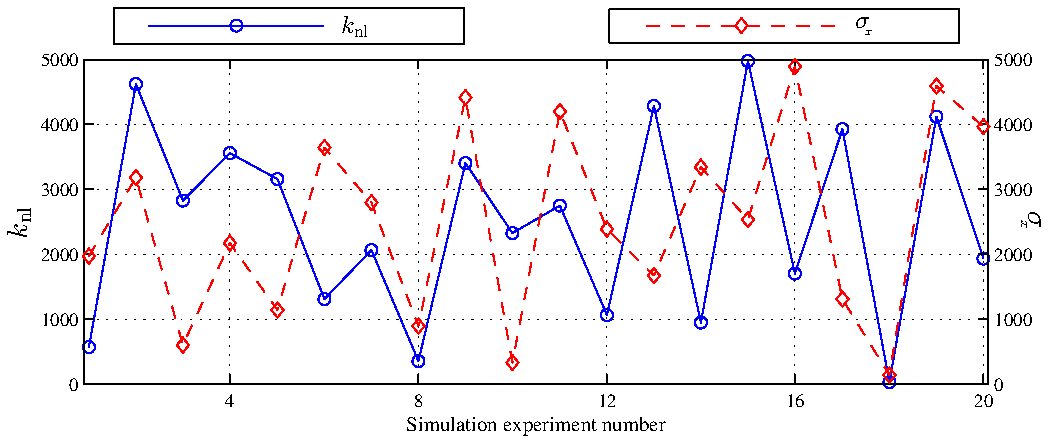
\includegraphics[width = 1\textwidth]{figs/cubic_uncprops.pdf}
\caption{Cubic stiffness coefficient $k_{nl}$ and excitation standard deviation $\sigma_x$ values for the 20 simulations conducted. \label{fig:cubic_uncprops}}
\end{center}
\end{figure}
% ================================================


The metamodeling method in this case focuses on the approximation of the dynamic response of the system under study in the discrete time domain by a PC-NARX model. The latter should be able to describe the system dynamics for the complete input variable space and of course to be much cheaper computationally. The estimation of the appropriate PC-NARX is based on the displacement responses of the system under study for 20 simulation experiments. The realizations of the uncertain input variables for these simulations are drawn by means of the LHS method and their values are illustrated in Fig. \ref{fig:cubic_uncprops}.     


A fourth-order Runge-Kutta scheme is used to obtain the response of the nonlinear system excited by Gaussian white noise sequences $x_k(t)$ ($k = 1, \ldots, 20, t = -7.5, \ldots, 5 $ s) with various std values and a frequency range from 0 to 20 Hz. The system's response was simulated with a sampling period of 0.005 s, that is a sampling frequency $f_s = 200$ Hz. In order to avoid the transient dynamic response the first 1500 samples of the response are discarded and thus the final set of simulated responses consists of 20 sets of 1000-sample vectors $y_k[t]$ ($k = 1, \ldots, 20, t = 1, \ldots, 1000 $).




% Table
% ================================================
\begin{table} 
\centering\begin{spacing}{1.25}
\caption{Computational and optimization methods used and algorithmic details.}\label{tab:alg_details}
\begin{tabular}{lll}\hline
Method & Matlab function & Algorithmic details \\ \hline
Numerical integration  & \multirow{2}{*}{\emph{ode45}} & \multirow{2}{*}{ RelTol = $ 10^{-4}$, AbsTol = $ 10^{-8}$} \\ 
(Runge-Kutta) & & \\ \hdashline
\multirow{2}{*}{Genetic Algorithm} & \multirow{2}{*}{\emph{ga}} & population size = 100, crossover fraction = 0.7, \\
& & mutation fraction = 0.3, elite count = 5 $\%$ \\ \hdashline
Linear least squares &  \emph{mldivide} & QR factorization \\ \hdashline
Nonlinear least squares  & \multirow{2}{*}{\emph{lsqnonlin}} & \multirow{2}{*}{TolFun = $ 10^{-3}$, TolX = $ 10^{-6}$}  \\ 
(Levenberg-Marquardt) & & \\\hline
\end{tabular}
\end{spacing}
\end{table}
% ================================================




The displacement-restoring force diagrams for two of the simulation experiments ($\#$18 and $\#$19) are depicted in Fig. \ref{fig:cubic_randexc}. For these simulation experiments the set of input variables are close to the bounds of their distribution, that is $\bxi_{18} = [k_{\mathrm{nl}} , \sigma_x]^T \simeq [29 , 136]^T $ and $\bxi_{19} \simeq [4114, 4586]^T $. Obviously, the system depicts an almost linear behaviour for $\bxi_{18} $, but highly nonlinear for $\bxi_{19}$. The latter set of input-output (force-displacement) signals is chosen for the nonlinear regressors selection below.   


% Figure
% ================================================
\begin{figure}[t!]
\begin{center}
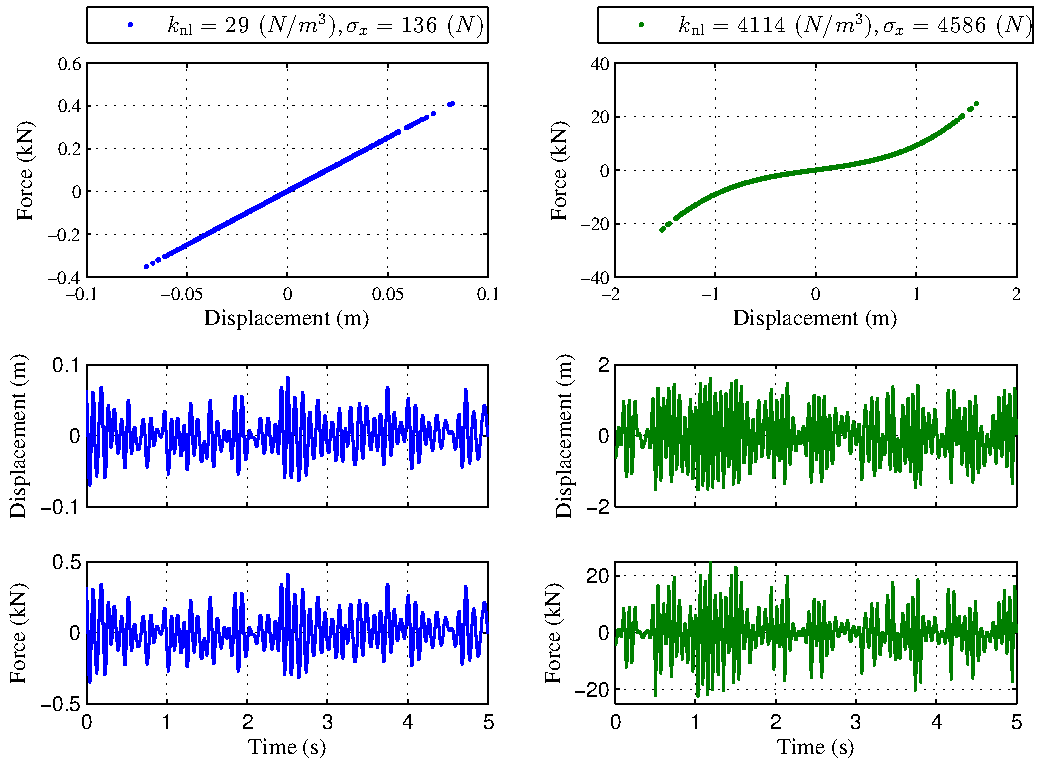
\includegraphics[width = 0.75\textwidth]{figs/cubic_randexci.pdf}
\caption{Cubic stiffness system displacement response versus restoring force for simulation experiments $\#$18 (left column) and $\#$19 (right column).\label{fig:cubic_randexc}}
\end{center}
\end{figure}
% ================================================

As long as the system under study has a single degree-of-freedom, PC-NARX models with $ n_a = n_b = 2 $ are considered, while the appropriate nonlinear terms $g_i({\bld z}[t])$ are probed from a pool of polynomial functions of the following form:
%
$$ g_i({\bld z}[t]) = z_{j}[t]^{\ell} $$
%
with $\ell \in \{0,1,2,3\}$, and ${\bld z}[t] = \left\{ \ y[t-1], y[t-2], x[t], x[t-1], x[t-2]\ \right\}^{T}$, leading to 16 candidate terms including the constant term.

The application of the GA for the selection of the most significant terms (see Table \ref{tab:alg_details} for algorithmic details), leads to the initial selection of 10 terms. However, the backward selection analysis may be utilized to further reduce the number of terms to four as shown in Fig. \ref{fig:cubic_MSS_A}. It is reminded that, within GA the candidate NARX models are estimated by the PE method but assessed with respect to their simulation capabilities evaluated by means of the normalized squared simulation error criterion:
%
\beq
\text{NSSE} =\frac{ \sum_{t=1}^N \left(y_k[t] - \tilde{y}_k[t]\right)^2 } {\sum_{t=1}^N y_k[t]^2}\ (\%) 
\eeq
%
Local NARX models with the selected regressors are then estimated for each of the simulation experiment.

  
% Figure
% ================================================
\begin{figure}[t!]
\begin{center}
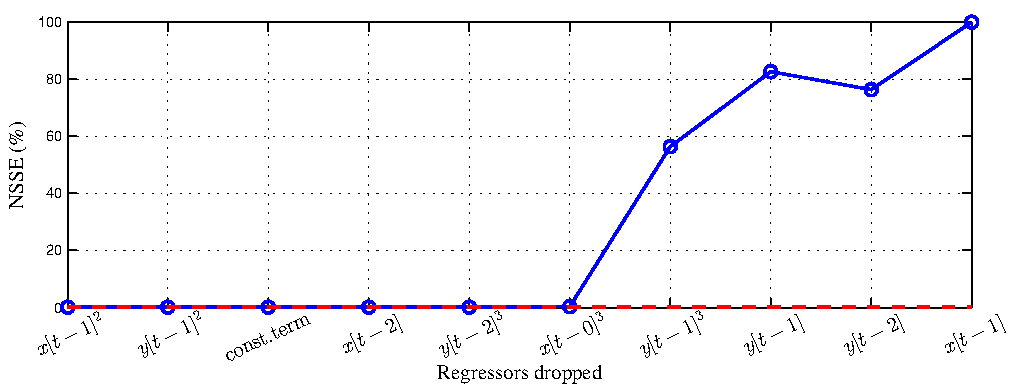
\includegraphics[width = 1\textwidth]{figs/cubic_MSS_StageA.pdf}
\caption{Cubic stiffness system metamodeling: Backward selection of the NARX regressors based on the normalized squared simulation error criterion (simulation experiment dataset $\#$19; initial regressors selected through GA with the corresponding NSSE value obtained being indicated by the red dashed-line). \label{fig:cubic_MSS_A}}
\end{center}
\end{figure}
% ================================================

Subsequently, the appropriate for the expansion of the local NARX model parameters $\vartheta_i(\bxi_k)$ PC subspace, is searched among the multivariate Legendre polynomial basis functions (due to the uniform distributions of the input variables) with maximum total degree equal to four ($P = 4$). Thus, the initial search space consists of 14 candidate basis functions plus the constant basis which is nonetheless excluded from the PC subspace selection procedure. The GA initially singled out 9 of these bases, while the backward selection procedure results shown in Fig. \ref{fig:cubic_MSS_B} indicate that the number of bases could be potentially lowered to 6. 


% Figure
% ================================================
\begin{figure}[t!]
\begin{center}
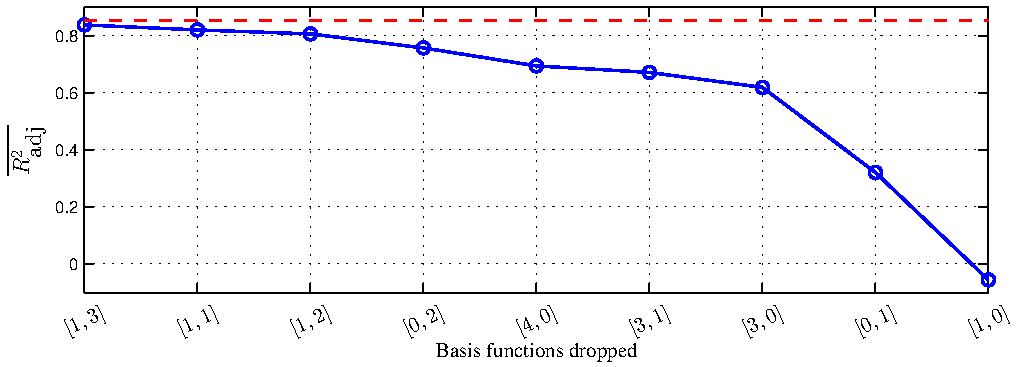
\includegraphics[width = 1\textwidth]{figs/cubic_MSS_StageB.pdf}
\caption{Cubic stiffness system metamodeling: Backward selection of the polynomial chaos functional subspace based on the mean adjusted $R^2$ criterion (maximum total polynomial degree $P=4$; initial subspace selected through GA with the corresponding $\overline{R^2_\text{adj}}$ value obtained being indicated by the red dashed-line).} \label{fig:cubic_MSS_B}
\end{center}
\end{figure}
% ================================================


% Table
% ================================================
\begin{table} 
\centering
\caption{Cubic stiffness system metamodeling: PC-NARX metamodel nonlinear regressors and PC basis functions multivariate indices.}\label{tab:PCNARXcubic}
\small \begin{tabular}{lc}\hline 
%\multicolumn{2}{l}{Geometric}& \multicolumn{2}{l}{Mechanical}\\[-6pt]
Nonlinear regressors & Polynomial Chaos \\
 & basis functions indices \\\hline
$g_1({\bld z}[t]) = x[t-1]$   	& ${\bld d}{(1)} = [0, 0]$ \\
$g_2({\bld z}[t]) = y[t-1]$   	& ${\bld d}{(2)} = [1, 0]$ \\
$g_3({\bld z}[t]) = y[t-2]$   	& ${\bld d}{(3)} = [0, 1]$ \\
$g_4({\bld z}[t]) = y[t-1]^3$ 	& ${\bld d}{(4)} = [0, 2]$ \\
 								& ${\bld d}{(5)} = [3, 0]$ \\
								& ${\bld d}{(6)} = [4, 0]$ \\
								& ${\bld d}{(7)} = [3, 1]$ \\ \hline
\end{tabular}
\end{table}
% ================================================



Therefore, the structure selection scheme leads to four nonlinear terms and seven PC basis functions, that is 28 coefficients of projection $\theta_{i,j}$. It may be observed that according to these results the PC-NARX metamodel parameters $\theta_i$ and thus the dynamic properties of the corresponding numerical model are found to be more sensitive to the input variable $k_{\mathrm{nl}}$ (see the multivariate indices of the PC basis in Fig. \ref{fig:cubic_MSS_B}). This fact is according to the expected result, since the nonlinear regressors selected through the PC-NARX metamodel structure selection scheme are those of the theoretical NARX model that is approximately describing the continuous system of Eqs. (\ref{eq:SDOF}) and (\ref{eq:cubic_restoring}). Indeed, the discretization of the nonlinear system may be realized by adopting a centered finite differencing method in order to approximate the derivative terms $\dot{y}(t)$ and $\ddot{y}(t)$, that is 
%
\begin{subequations}
%
\beq \dot{y}(t) \approx \frac{y(t+T_s) - y(t-T_s)}{2T_s} + O(T_s)\eeq
%
and
%
\beq \ddot{y}(t) \approx \frac{y(t+T_s) - 2y(t) + y(t-T_s)}{T_s^2} + O(T_s)\eeq
%
\end{subequations}
%
where $O(T_s)$ is the order of the truncation error, and $T_s$ is reminded that designates the sampling period. Using this scheme, the following discrete-time model may be used for the representation of the cubic stiffness system:   
%
\beq y[t] + \frac{k-\frac{2m}{T_s^2}}{L}y[t-1] + \frac{\frac{m}{T_s^2}-\frac{c}{2T_s}}{L}y[t-2] + \frac{k_{\mathrm{nl}}}{L}y^3[t-1] = \frac{1}{L}x[t-1], \quad \text{with } L = \left(\frac{m}{T_s^2}+\frac{c}{2T_s}\right) \label{eq:cubic_theor}\eeq
%
which corresponds to a NARX model with three linear and one nonlinear regressor, with parameters which depend only on the system's physical characteristics. Comparison, between the theoretical curve of this NARX model parameter and the corresponding PC-NARX metamodel parameter in Fig. \ref{fig:cubic_surfs} shows the excellent agreement of the SE-based estimated value. It should be noted that the regressors of the PC-NARX not included in the theoretical model of Eq. (\ref{eq:cubic_theor}), may be considered as higher order approximation terms.


% Figure
% ================================================
\begin{figure}[t!]
\centering{
\begin{picture}(470,175)
\put(0,0){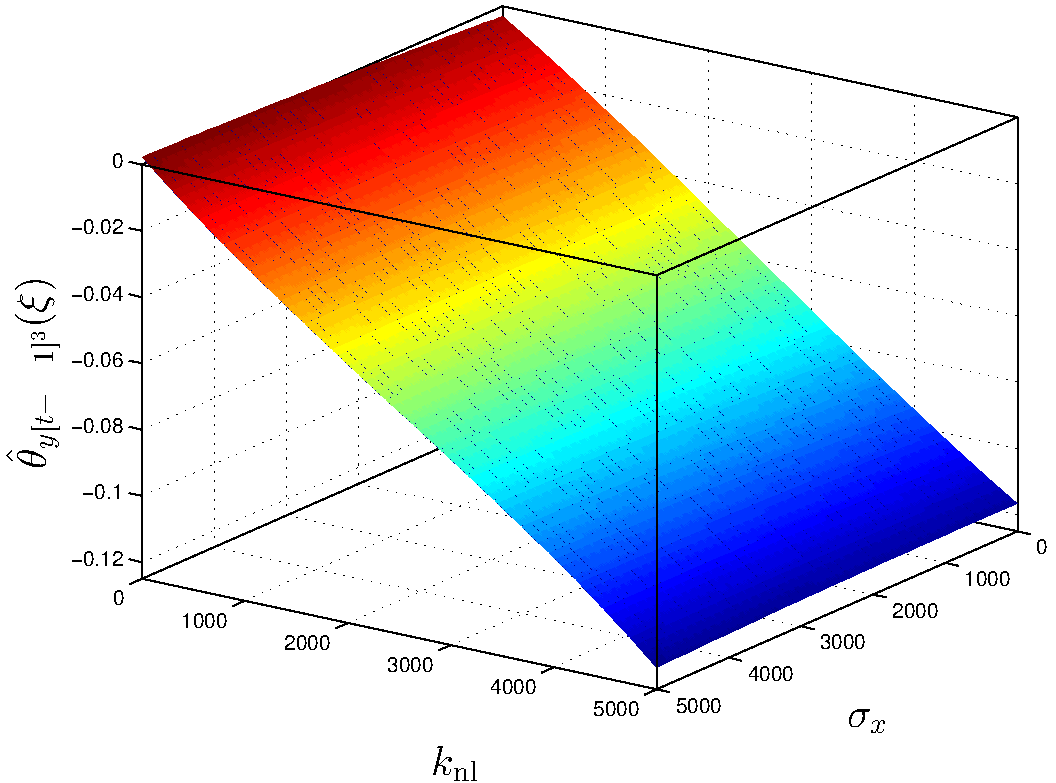
\includegraphics[width = 0.5\textwidth]{figs/cubic_surf.pdf}}
\put(240,0){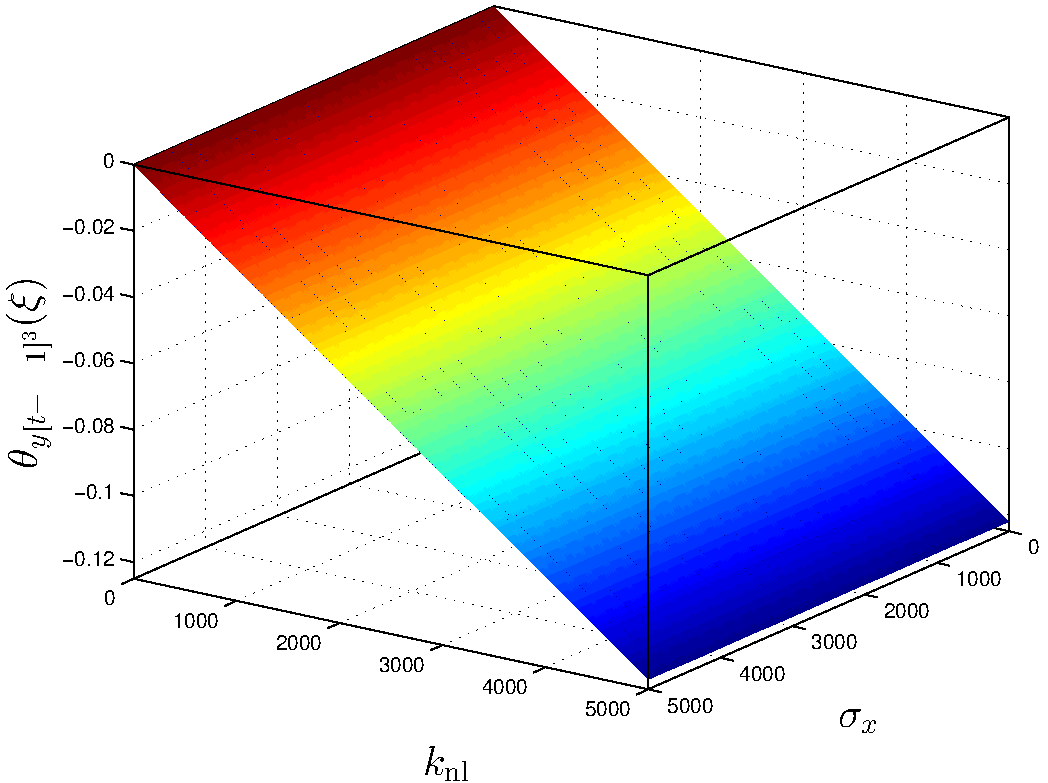
\includegraphics[width = 0.5\textwidth]{figs/cubic_surf_theor.pdf}}
\put(0,160){(a)}
\put(240,160){(b)}
\end{picture}}
\caption{Cubic stiffness system metamodeling: (a) SE-based PC-NARX metamodel parameter $\theta_{y[t-1]^3}(\bxi)$ as a function of $k_{\mathrm{nl}}$ and $\sigma_x$, and (b) the corresponding parameter of a NARX model computed directly by the difference scheme of the analytical differential equation describing the SDOF system.
\label{fig:cubic_surfs}}
\end{figure}
% ================================================



Finally, the estimated PC-NARX metamodel is validated through its usage for the simulation of 2 new input variable vectors which where not used during the PC-NARX model structure and estimation procedure. The simulated responses of the numerical model and those of the PC-NARX metamodel for these sets and an equal number of given realizations of the random process describing the excitation force, are contrasted in Fig. \ref{fig:cubic_validation}. The excellent agreement between the two simulated responses is apparent, while even if the purpose of this example is just illustrative, it should be mentioned that the integration with Runge-Kutta scheme takes close to 0.965 s for each simulation experiment while the PC-NARX metamodel needs approximately 0.143 s (mean values obtained from 100 MATLAB runs on a PC with quad-core at 3.5 GHz Intel Xeon CPU, and 64-bit OS which was used during all simulation experiments).



% Figure
% ================================================
\begin{figure}[t!]
\begin{center}
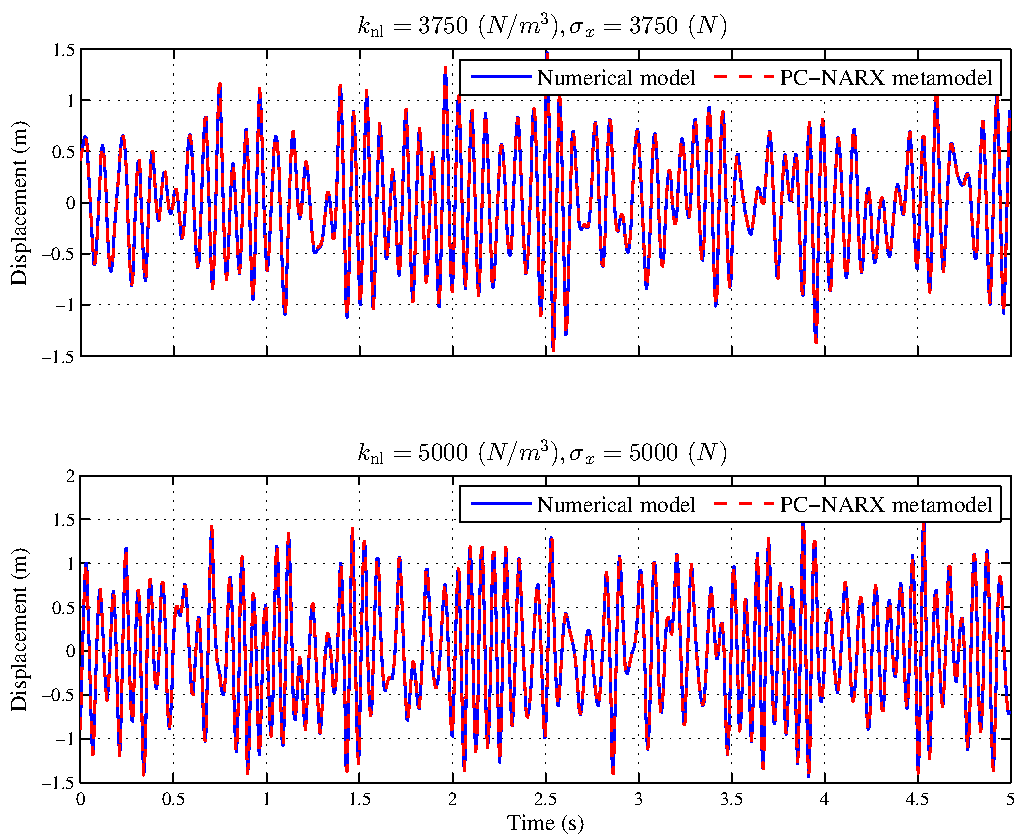
\includegraphics[width = 0.75\textwidth]{figs/cubic_randexci_val.pdf}
\caption{Cubic stiffness system PC-NARX metamodel validation: PC-NARX metamodel simulation contrasted to the simulations of the numerical model for (a) $k=3750,\sigma_x = 3750$, and (b) $k = 5000,\sigma_x = 5000$. 
\label{fig:cubic_validation}}
\end{center}
\end{figure}
% ================================================ 






% ================================================
\subsubsection{Hysteretic system}
% ================================================

The system considered in this case is a hysteretic dissipative system described by a Bouc-Wen type restoring force: 
%
\beq F(t) = \alpha k {y}(t) + (1-\alpha)k {z}(t) \eeq
%
with \beq \dot{z}(t) = A \dot{y}(t) + \beta |\dot{y}(t)| | z(t)|^{n-1} z(t) - \gamma\dot{y}(t) | z(t)|^{n}  \eeq
%
$\alpha$ designating the post- to pre-yield stiffness $k$, and $A$, $\beta>0$, $\gamma$ and $n$ the dimensionless quantities controlling the shape of the hysteresis loop \cite{Ismail-etal2009}. The nonlinear SDOF system is again considered to be subject to stationary random forces with uncertain standard deviation, while it is also characterized by uncertainty of the parameter $\beta$. The properties of the system are summarized in Table \ref{tab:boucwen_prop}.   


% Table
% ================================================
\begin{table} 
\centering
\caption{Properties of the SDOF system with hysteretic restoring force.}\label{tab:boucwen_prop}
\begin{tabular}{ll}\hline
mass & $m = 1$ kg \\
damping coefficient & $c = 0 $ N/ (m/s) \\
linear stiffness coefficient & $k = 50 $ N/m\\
post- to preyield stiffness ratio & $\alpha = 0 $ \\
hysteretic loop shape parameters & $ A = 1, \gamma = 0, n = 3, \beta \sim {\cal U}(0,1) $ \\
excitation force & $x \sim NID(0,\sigma_x^2)$ with $\sigma_x \sim {\cal U}(0,100) $ \\ \hline
\end{tabular}
\end{table}
% ================================================



Also in this case, the estimation of the PC-NARX metamodel is based on 20 simulation experiments, for which the samples of the uncertain input variables, drawn by means of the LHS method, are as shown in Fig.\ref{fig:boucwen_uncprops}. The numerical integration method and the algorithmic details are as in the previous example.

% Figure
% ================================================
\begin{figure}[t!]
\begin{center}
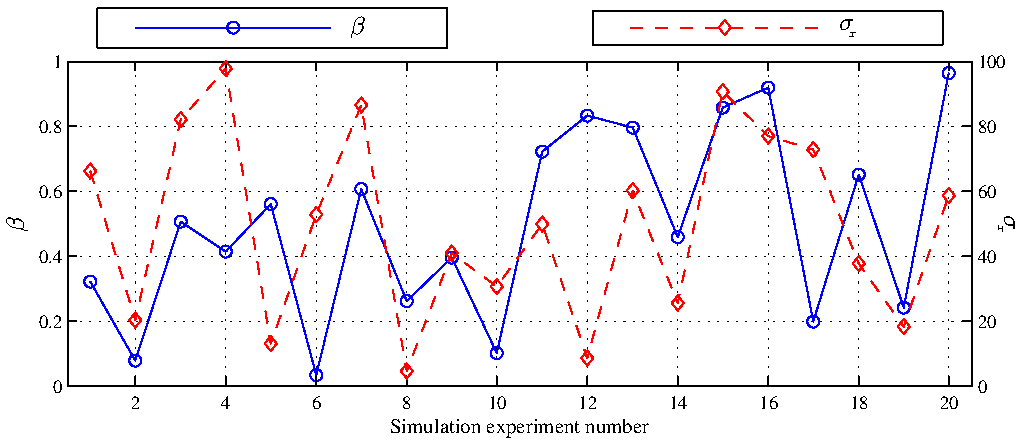
\includegraphics[width = 1\textwidth]{figs/boucwen_uncprops.pdf}
\caption{Bouc-Wen model parameter $\beta$ and excitation standard deviation $\sigma_x$ values for the 20 simulations conducted. \label{fig:boucwen_uncprops}}
\end{center}
\end{figure}
% ================================================


The displacement-restoring force diagrams for two of the simulation experiments ($\#2$ and $\#15$) are depicted in Fig. \ref{fig:boucwen_randexc}. For these simulation experiments the sets of input variables are $\bxi_2 = [\beta , \sigma_x]^T \simeq [ 0.08, 20]^T $ and $\bxi_{15} \simeq [0.86 , 91]^T $, and obviously a range of behaviours from almost linear to highly nonlinear may be observed depending on the sampled values of the uncertain input variables.

% Figure
% ================================================
\begin{figure}[t!]
\begin{center}
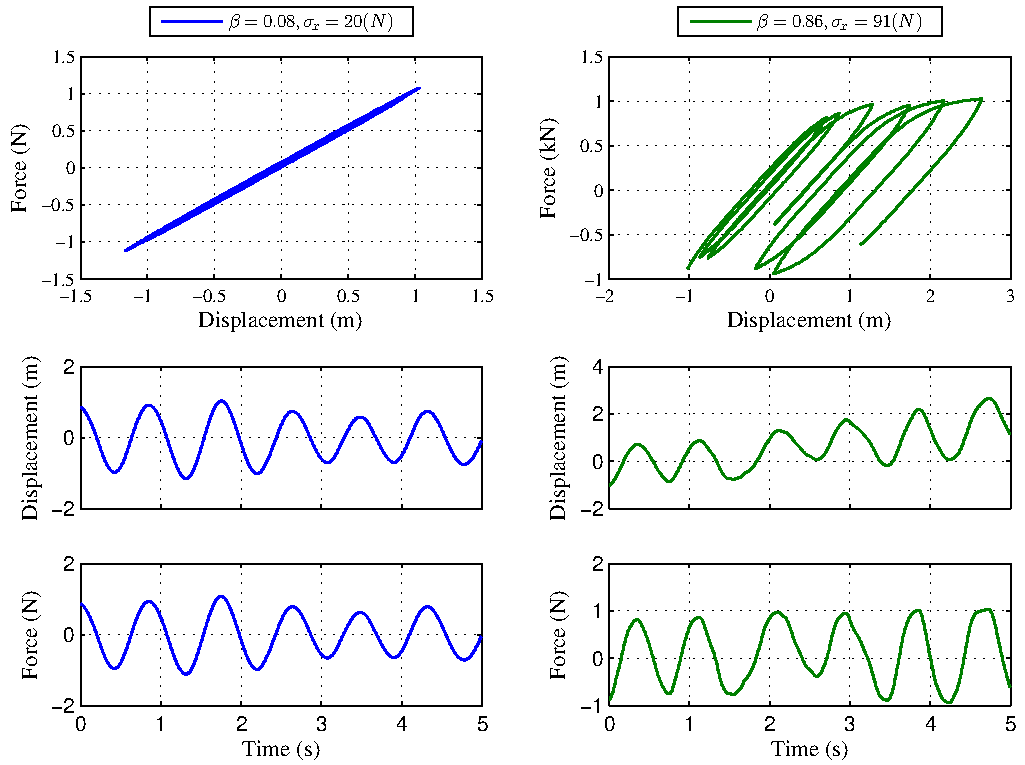
\includegraphics[width = 0.85\textwidth]{figs/boucwen_randexci.pdf}
\caption{Hysteretic system displacement response versus restoring force for simulation experiment $\#2$ (left column) and $\#15$ (right column). \label{fig:boucwen_randexc}}
\end{center}
\end{figure}
% ================================================

The metamodeling of this SDOF system is based on the simulated velocity responses, since it is simpler to describe such a system by a single ODE with respect to velocity \cite{Worden-Barthorpe2012}. By using a finite differencing method this ODE may be approximately represented by a NARX model in the discrete time domain (for example see the analysis in \cite{Worden-Barthorpe2012}). However, the nonlinear regressors of this NARX model would be of the following general form:
%
$$ g_i({\bld z}[t]) = z_{j_1}[t]^{\ell_1} \cdot z_{j_2}[t]^{\ell_2} \cdot z_{j_3}[t]^{\ell_3} \cdot |y[t-1]|^{\ell_4}$$
%  
with $\{\ell_1,\ell_2,\ell_3\} \in \{0,1,2,3\}$ and $ \ell_1 + \ell_2 + \ell_3 <= 3 $, $\ell_4 \in\{ 0,1 \}$ and ${\bld z}[t] = \left\{ \ y[t-1], y[t-2], x[t], x[t-1], x[t-2]\ \right\}^{T}$, with the absolute function being included due to the nature of the physical, i.e. hysteresis, problem. Adopting the above form to describe the initial search space for the PC-NARX nonlinear regressors selection, leads to 111 candidate terms including the constant term; a rather large number considering that the metamodeling procedure concerns an SDOF system. 

In order to simplify the metamodeling procedure and assess the applicability of the method for cases in which the nonlinear regressor search space is not appropriately selected, either due to lack of physical insight to the nonlinear mechanism or due to truncation of excessive spaces, the candidate regressors are considered to be of the simpler following form:
%
$$ g_i({\bld z}[t]) = z_{j_1}[t]^{\ell_1} \cdot |y[t-1]|^{\ell_2}$$
%  
with $ \ell_1 \in \{0,1,2,3\}$, $\ell_2 \in\{ 0,1 \}$ and ${\bld z}[t] = \left\{ \ y[t-1], y[t-2], x[t], x[t-1], x[t-2]\ \right\}^{T}$, resulting to a pool of 31 candidate terms.    


% Figure
% ================================================
\begin{figure}[t!]
\begin{center}
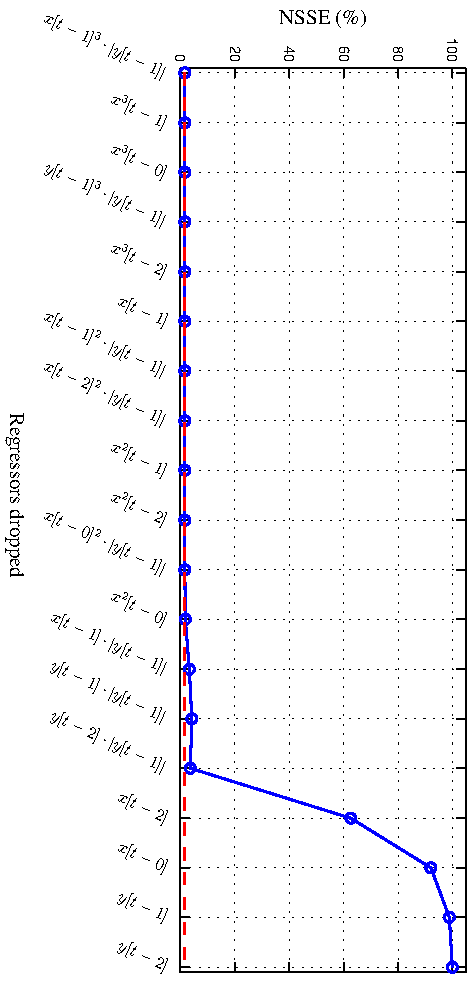
\includegraphics[height = 1\textwidth, angle = 90]{figs/boucwen_MSS_StageA.pdf}
\caption{Hysteretic system metamodeling: Backward selection of the NARX regressors based on the normalized squared simulation error criterion (simulation experiment dataset $\#$15; initial regressors selected through GA with the corresponding NSSE value obtained being indicated by the red dashed-line).} \label{fig:boucwen_MSS_A}
\end{center}
\end{figure}
% ================================================


% Figure
% ================================================
\begin{figure}[t!]
\begin{center}
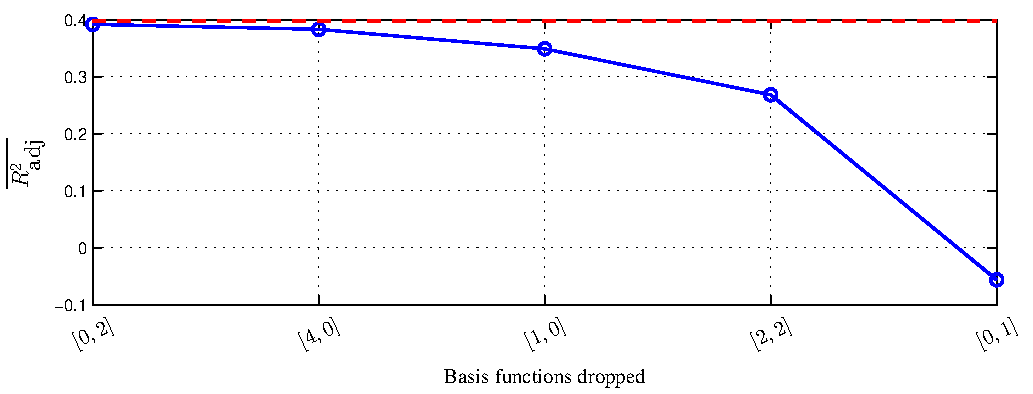
\includegraphics[width = 1\textwidth]{figs/boucwen_MSS_StageB.pdf}
\caption{Hysteretic system metamodeling: Backward selection of the polynomial chaos functional subspace based on the mean adjusted $R^2$ criterion (maximum total polynomial degree $P=4$; initial subspace selected through GA with the corresponding $\overline{R^2_\text{adj}}$ value obtained being indicated by the red dashed-line).} \label{fig:boucwen_MSS_B}
\end{center}
\end{figure}
% ================================================


The initial global search performed by the GA for the input-output (force-velocity) dataset of simulation experiment $\#15$, leads to an initial selection of 19 nonlinear terms, which may further be reduced to 7 by backward selection (see results in Fig. \ref{fig:boucwen_MSS_A}). Employing these terms, local NARX models are estimated for each one of the 20 simulation experiments. The resulting NARX model parameters are expanded on a PC subspace which is selected by the procedure described in Section \ref{sec:MSS}. The initial selection of the maximum total degree $P=4$ and the GA optimization indicated a PC basis consisting of 5 basis functions, while this number may be potentially reduced to 3 after the backward selection procedure (see Fig. \ref{fig:boucwen_MSS_B}). The nonlinear regressors and the multivariate basis indices finally selected for the PC-NARX metamodel of the hysteretic system are summarized in Table \ref{tab:PCNARXboucwen}. Two of the estimated PC-NARX parameters, namely $\hat{\theta}_4(\bxi)$ and $\hat{\theta}_{7}(\bxi)$ corresponding to the nonlinear regressor terms $y[t-2]$ and $y[t-2]\! \cdot\!  |y[t-1]|(\bxi)$ respectively, are plotted as a function of both input variables $\beta$ and $\sigma_x$ in Fig. \ref{fig:boucwen_surfs}.


% Figure
% ================================================
\begin{figure}[t!]
\centering{
\begin{picture}(450,170)
\put(0,0){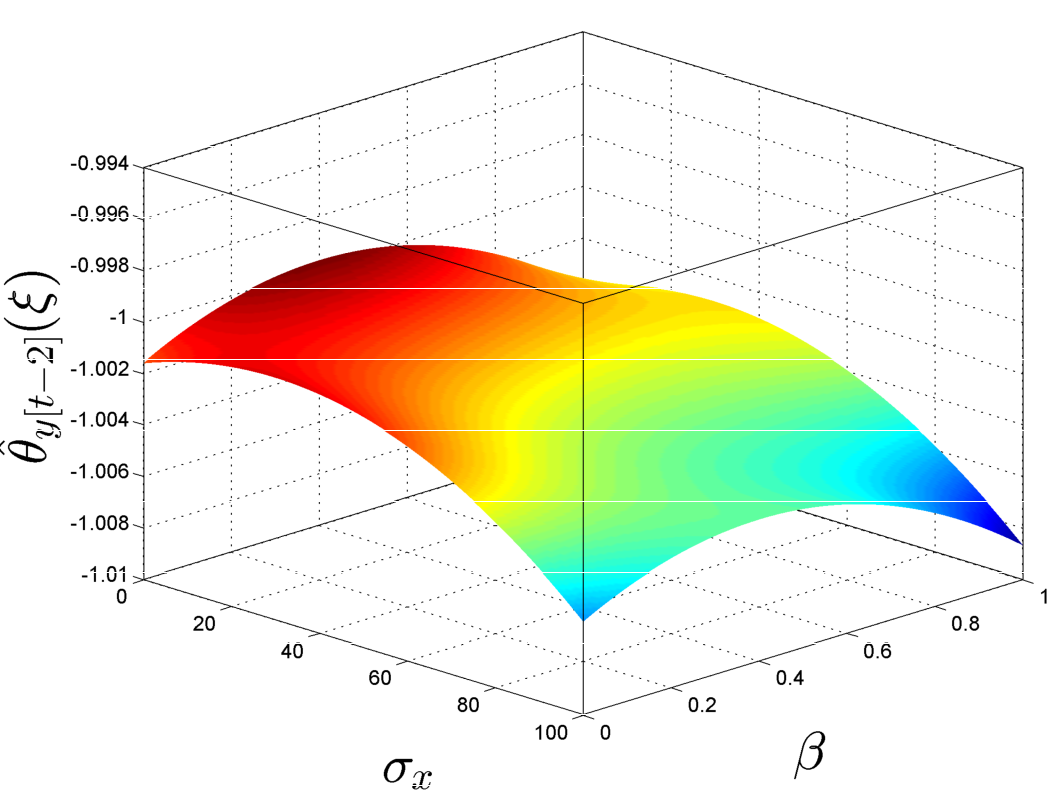
\includegraphics[width = 0.475\textwidth]{figs/boucwen_surf_b.pdf}}
\put(225,0){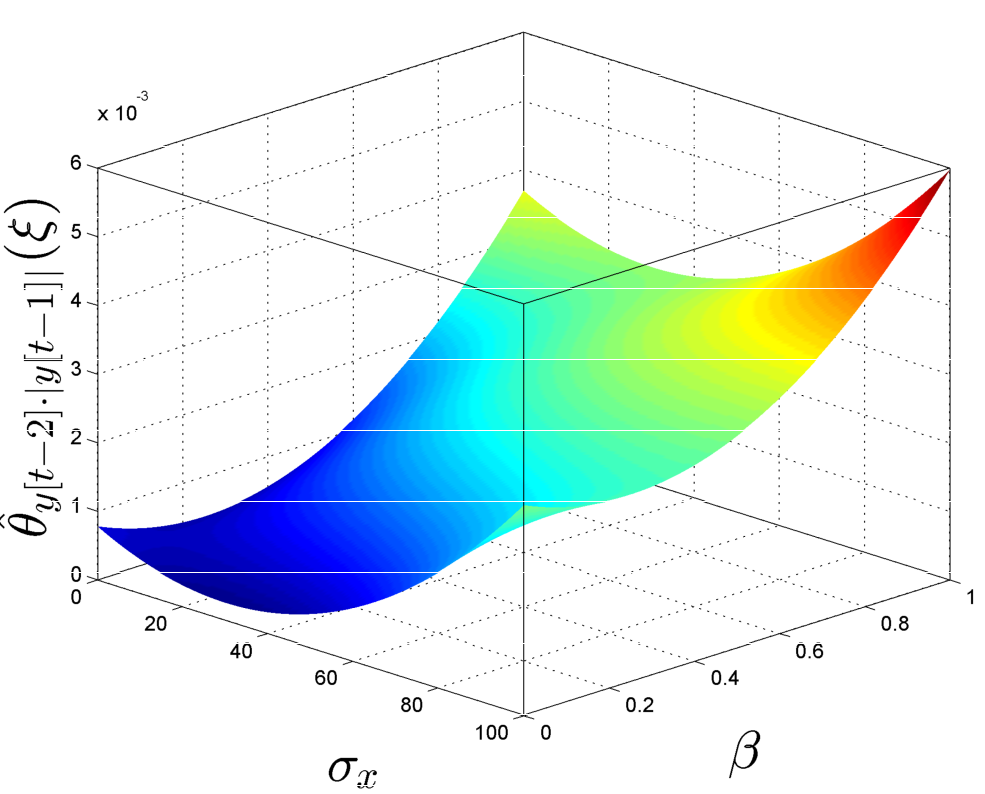
\includegraphics[width = 0.475\textwidth]{figs/boucwen_surf_a.pdf}}
\put(0,160){(a)}
\put(225,160){(b)}
\end{picture}}
\caption{Hysteretic system metamodeling: (a) $\hat{\theta}_{y[t-2]}(\bxi)$, and (b) $\hat{\theta}_{y[t-2]\cdot |y[t-1]|}(\bxi)$ SE-based PC-NARX metamodel parameter estimates as a function of $\beta$ and $\sigma_x$.}
\label{fig:boucwen_surfs}
\end{figure}
% ================================================


% Table
% ================================================
\begin{table} 
\centering
\caption{Hysteretic system PC-NARX metamodel nonlinear regressors and PC basis functions multivariate indices.}\label{tab:PCNARXboucwen}
\small \begin{tabular}{lc}\hline 
%\multicolumn{2}{l}{Geometric}& \multicolumn{2}{l}{Mechanical}\\[-6pt]
Nonlinear regressors & Polynomial Chaos \\
 & basis functions indices \\\hline
$g_1({\bld z}[t]) = x[t]$ & ${\bld d}{(1)} = [0, 0]$ \\
$g_2({\bld z}[t]) = x[t-2]$ & ${\bld d}{(2)} = [1, 0]$ \\
$g_3({\bld z}[t]) = y[t-1]$ & ${\bld d}{(3)} = [0, 1]$ \\
$g_4({\bld z}[t]) = y[t-2]$ & ${\bld d}{(4)} = [2, 2]$ \\
$g_5({\bld z}[t]) = x[t-1] \cdot |y[t-1]|$ & \\
$g_6({\bld z}[t]) = y[t-1] \cdot |y[t-1]|$ & \\
$g_7({\bld z}[t]) = y[t-2] \cdot |y[t-1]|$ & \\ \hline
\end{tabular}
\end{table}
% ================================================

 
It should be noted, that the NSSE criterion values obtained by the estimated PC-NARX models are lower than 3.1 $\%$ for all 20 simulation experiments of the estimation set -- 18 of them are less than 1 $\%$ -- while similar performance is succeeded for input variable vectors not included in the estimation set. For example, the simulated responses of the numerical model and those of the PC-NARX metamodel for two input variable vectors ($\bxi_{1}^{\text{valid}} = [0.25, 0.5]$ and $\bxi_{2}^{\text{valid}} = [\beta, \sigma_x] = [1, 100]$) are contrasted in Fig. \ref{fig:boucwen_validation}. As it may be observed, the PC-NARX metamodel achieves very good simulation performance (NSSE equals to 0.25 \% and 0.99 \% respectively).


% Figure
% ================================================
\begin{figure}[t!]
\begin{center}
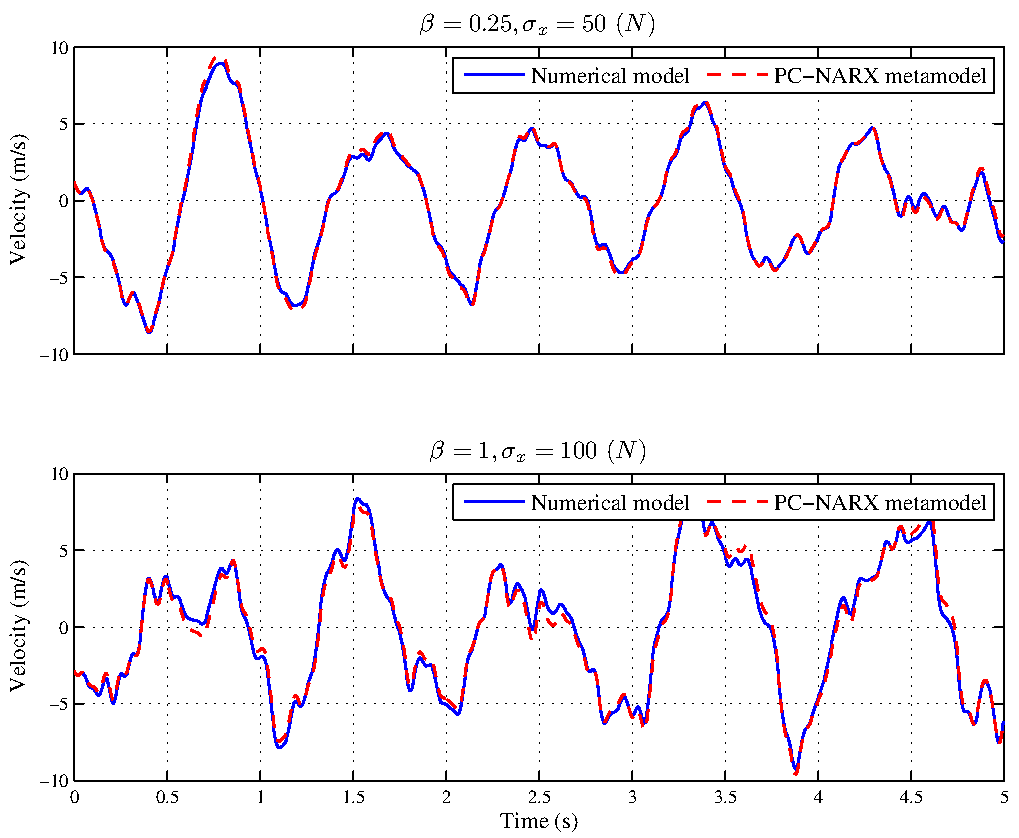
\includegraphics[width = 0.75\textwidth]{figs/boucwen_randexci_val.pdf}
\caption{Hysteretic system PC-NARX metamodel validation: PC-NARX metamodel simulation contrasted to the simulations of the numerical model for (a) $ \beta = 0.25,\sigma_x = 50$, and (b) $ \beta = 1,\sigma_x = 100$. 
\label{fig:boucwen_validation}}
\end{center}
\end{figure}
% ================================================ 





% ================================================
\subsection{Multi-storey steel frame model}
% ================================================
A FE model of a multi-storey three-bay frame of a building structure (Fig. \ref{fig:SteelFrame}) subject to base acceleration excitation ($x[t] =\alpha_{g}[t] $) is presently considered for the assessment of the introduced method. The elements of the shear frame are considered to have square cross section of width $w$, being made of steel with isotropic behavior described by a bilinear stress-strain curve. The values of the mechanical and geometric properties of the structure are summarized in Table \ref{tab:con_prop}. It is considered that the steel's Young modulus $E$ is characterized by uncertainty that may be modelled by a random variable following a normal distribution $ E \sim {\mathcal N}(200,16)$ GPa. The rest of the model's mechanical and geometric properties are considered to be characterized by negligible uncertainty.


% Figure
% ================================================
\begin{figure}[t]
\centering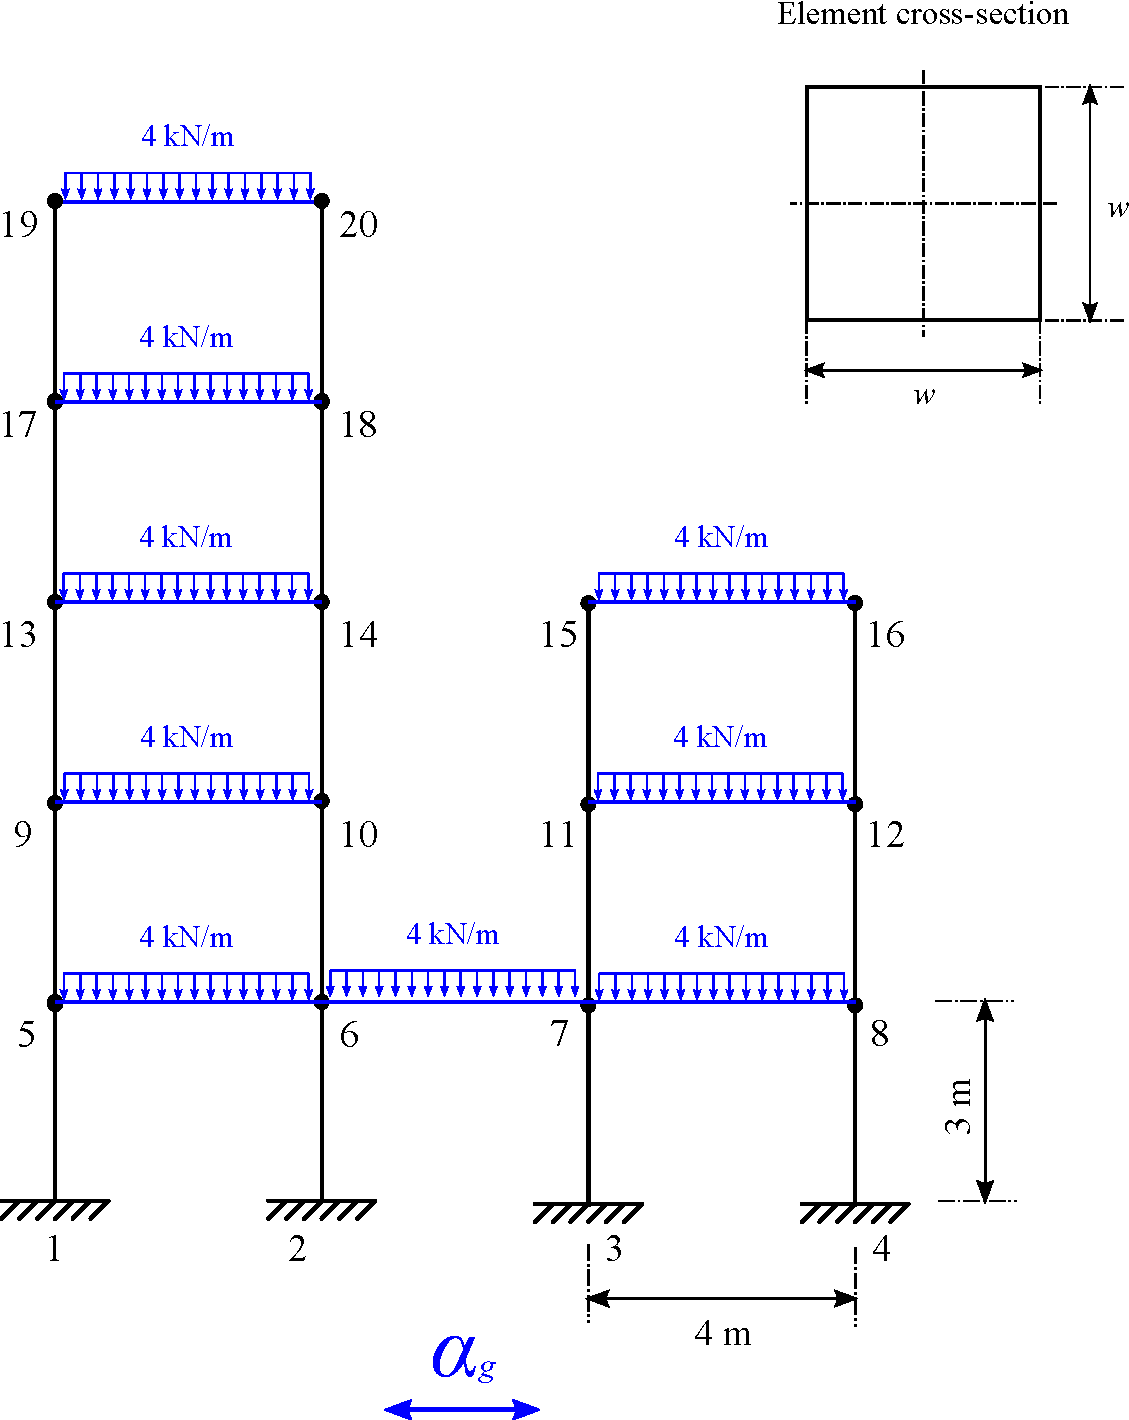
\includegraphics[width = 0.5\textwidth]{figs/multistoreySF.pdf}
\caption{The multi-storey shear frame building model.}\label{fig:SteelFrame}
\end{figure}
% ================================================

% Table
% ================================================
\begin{table} 
\centering
\caption{The values of the geometric and mechanical properties of the multi-storey frame model.}\label{tab:con_prop}
\begin{tabular}{lcll}\hline
\multicolumn{2}{l}{Geometric}& \multicolumn{2}{l}{Mechanical}\\[-6pt]
\multicolumn{2}{l}{\hrulefill}& & \\
Cross-section width & \hspace{-0.2cm} m & & \\\hline
1$^{\text{st}}$ storey columns & \hspace{-0.2cm} $w_{c_1} =$ 0.200  & Poisson ratio & \hspace{-0.2cm} $\nu=$ 0.29 \\
2$^{\text{nd}}$ storey columns & \hspace{-0.2cm} $w_{c_2} =$ 0.175  & Density & \hspace{-0.2cm} $ \rho =$ 7850 (kg/m$^3$)\\
3$^{\text{rd}}$ storey columns & \hspace{-0.2cm} $w_{c_3} =$ 0.150  & Young modulus & \hspace{-0.2cm} $ E \sim {\cal N}(200,16) $ (GPa) \\
4$^{\text{th}}$ storey columns & \hspace{-0.2cm} $w_{c_4} =$ 0.125  & Yield stress & \hspace{-0.2cm} $ \sigma_Y = $ 200 (MPa)\\
5$^{\text{th}}$ storey columns & \hspace{-0.2cm} $w_{c_5} =$ 0.100  & Tangent modulus & \hspace{-0.2cm} $ E_T = $ 20 (GPa) \\
Horizontal beams & \hspace{-0.2cm} $w_{h}=$ 0.150 & & \\\hline
\end{tabular}
\end{table}
% ================================================

The frame model is considered to be subject to Gaussian white noise base acceleration excitation applied in x-axis direction (1000 samples, sampling frequency $f_s = 50$ Hz). The input excitation has zero mean value and uncertain standard deviation $\sigma_a$ that follows a log-normal distribution with mean value equal to $2.5$ and standard deviation equal to $0.5$, that is $\sigma_\alpha \sim \ln {\cal N} (2.5,0.5)$.


A total number of $K = 20$ simulations are conducted for a corresponding number of input variable vectors $\bxi_k (k=1,2,\ldots,20)$ which are drawn by using the LHS method. The values of the input variables drawn are shown in Figure \ref{fig:mprops}.

% Figure
% ================================================
\begin{figure}[t!]
\begin{center}
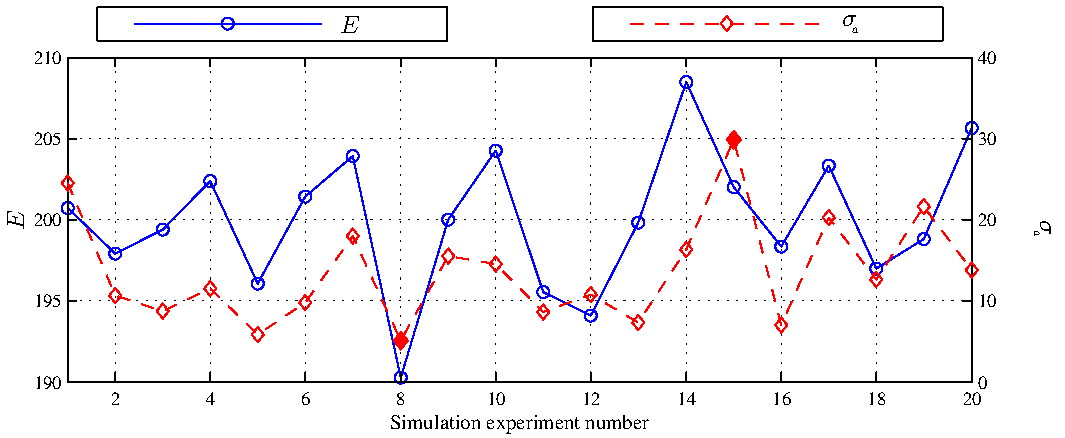
\includegraphics[width = 1\textwidth]{figs/SF_unprops.pdf}
\caption{Material properties and standard deviation of the input acceleration of the shear frame model for the 20 simulations conducted. \label{fig:mprops}}
\end{center}
\end{figure}
% ================================================

The time-histories of the model's displacement response as calculated by the FE model for node 7 versus the total reaction base force for the simulations with the input excitation lowest standard deviation value (simulation experiment $\#8$) and the highest standard deviation value (simulation experiment $\#15$) are shown in Figure \ref{fig:SF_randexc}. As expected, significant differences between the two datasets may be readily observed, fact that may attributed to the amplitude of excitation which as becomes higher excites the nonlinear dynamics of the modelled structure.


% Figure
% ================================================
\begin{figure}[t!]
\begin{center}
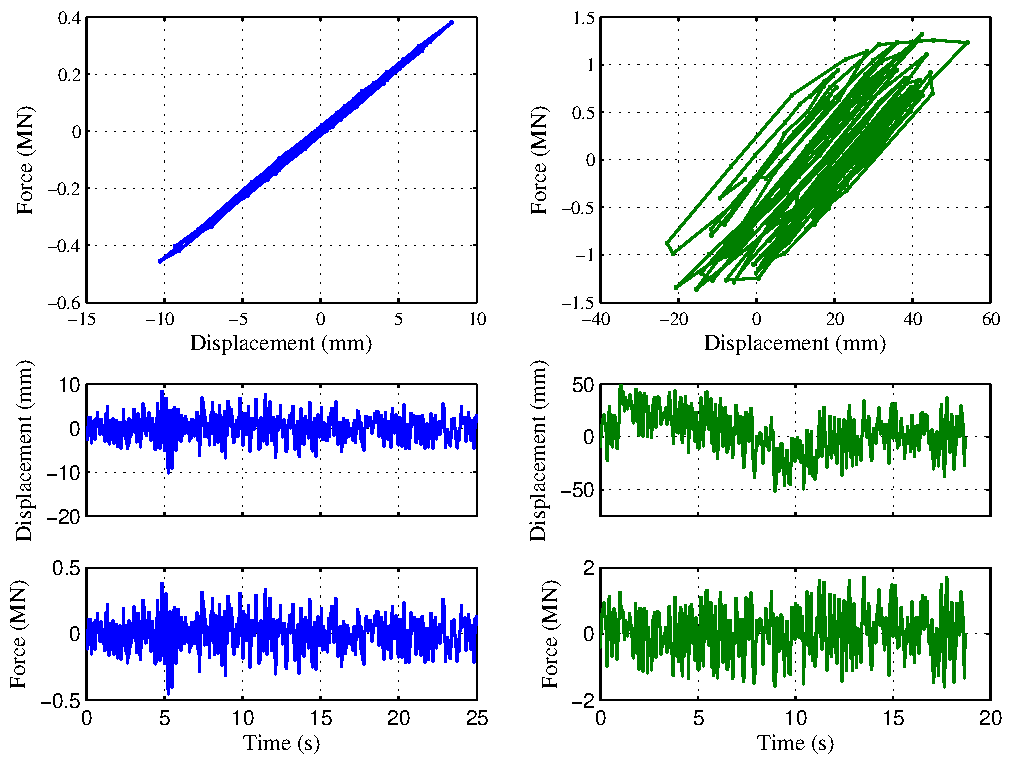
\includegraphics[width = 0.85\textwidth]{figs/SF_randexci.pdf}
\caption{FE model displacement response measured at node 7 versus total reaction base force for simulation experiment $\#8$ (left column) and $\#15$ (right column). \label{fig:SF_randexc}}
\end{center}
\end{figure}
% ================================================


The identification of the frame's metamodel is based on recordings of the horizontal velocity of the first floor of the frame measured at node 7 ($y[t] = v_{7}[t] $). In order to avoid the transient effects, the first 200 samples of the input excitation and the corresponding dynamic response signals of the frame are excluded from the PC-NARX metamodeling procedure.  

For the PC-NARX metamodeling problem, the orders $n_a$ and  $n_b$ are considered equal to 14 since the shear frame may be approximated by a seven DOF system, while the appropriate nonlinear regressors are searched among functions of the following form: 
%
$$ g_i({\bld z}[t]) = z_{j}[t]^{\ell_1} \cdot |y[t - \ell_2]|^{\ell_3}$$
%  
with ${\bld z}[t] = \left\{ \ y[t-1], y[t-2],\ldots,y[t-14], x[t], x[t-1],x[t-2] ,\ldots, x[t-14]\ \right\}^{T}$, $\ell_1 \in \{1,2,3\}$, $\ell_2 \in\{ 1,\ldots,7 \}$, and $\ell_3 \in\{ 0,1 \}$, leading to 697 candidate terms including the constant function. The absolute function is again incorporated in the functions above since the bilinear material behaviour is expected to add hysteresis phenomena into the dynamics of the modeled structure.  

The nonlinear regressors of the PC-NARX metamodel are first selected by using the GA-based procedure and the simulated response data ${\bld y}_{15}^N$ which corresponds to the base excitation with the highest standard deviation. GA optimization distinguishes 411 terms as appropriate for the NARX model to represent the system dynamics for $\bxi_{15}$. The backward selection results shown in Fig. \ref{fig:SF_MSS_A} highlight the fact that for more complex systems and initial search spaces which do not necessarily include the actual nonlinear functions representing the numerical model, the selection of the appropriate nonlinear terms is a difficult decision. In this test case, only the last 93 terms are retained which provided NSSE lower than 2 $\%$, with this choice being by no means compulsory, but having to do with the desired level of approximation accuracy.  

% Figure
% ================================================
\begin{figure}[t!]
\begin{center}
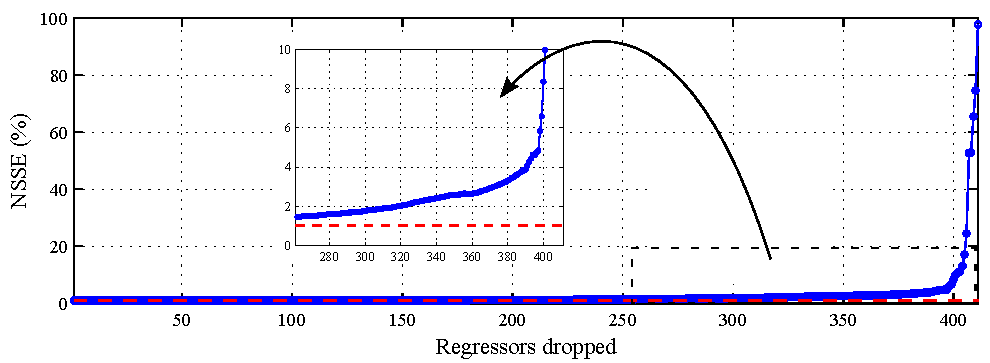
\includegraphics[width = 1\textwidth]{figs/multi_MSS_StageA.pdf}
\caption{Shear frame FE model metamodeling: Backward selection of the NARX regressors based on the normalized squared simulation error criterion (simulation experiment dataset $\#$15; initial regressors selected through GA with the corresponding NSSE value obtained being indicated by the red dashed-line).} \label{fig:SF_MSS_A}
\end{center}
\end{figure}
% ================================================


% Figure
% ================================================
\begin{figure}[t!]
\begin{center}
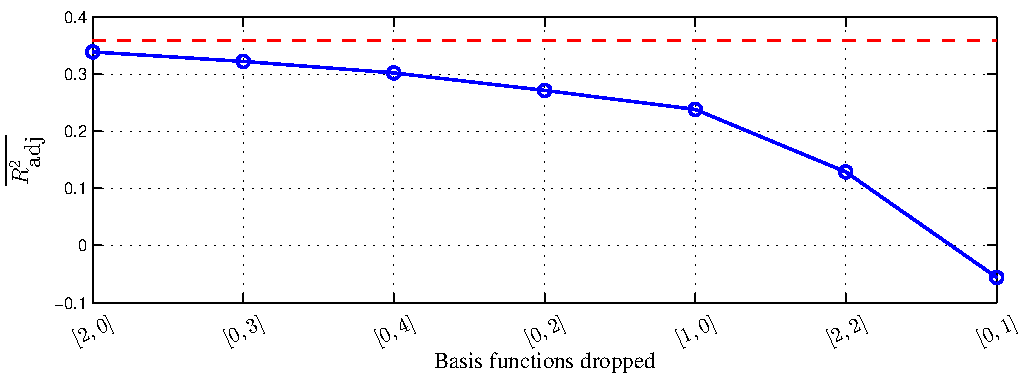
\includegraphics[width = 1\textwidth]{figs/SF_MSS_StageB.pdf}
\caption{Shear frame FE model metamodeling: Backward selection of the polynomial chaos functional subspace based on the mean adjusted $R^2$ criterion (maximum total polynomial degree $P=4$; initial subspace selected through GA with the corresponding $\overline{R^2_\text{adj}}$ value obtained being indicated by the red dashed-line).} \label{fig:boucwen_MSS_B}
\end{center}
\end{figure}
% ================================================


The input random variables are transformed into standard normal variables with the NARX coefficient being expanded on Hermite polynomials of the standard normal random variables $\xi_1$, and $\xi_2$:
%%
\beq \xi_1 =  \frac{E - 200}{16} , \quad \xi_2 =  \frac{\exp(\sigma_a) - 2.5}{0.5}\eeq 
%%
The GA-based selection of the PC subspace gives 7 basis functions for $P = 4$. The backward selection scheme is then employed in order to investigate the potentiality of reducing the initial subspace. Nevertheless, based on Fig. \ref{fig:cubic_MSS_B} none of the initially selected basis functions is discarded.   
 
The final set of (93 $\times$ 8) PC projection coefficients may be used for the simulation of the dynamic response of the FE model $y^N(\bxi)$ for any realization of $\bxi$ drawn from the predetermined joint pdf. The NSSE values of the reconstructed 20 signals that were used for the identification of the metamodel are lower than 2.6 \%. 

The performance of the estimated metamodel is finally assessed through its application for the simulation of the dynamic response of the numerical model of Figure \ref{fig:SteelFrame} for random variable values $\bxi^{\text{valid}}_j$ different from those of the initial 100 experiments. The simulated responses of the metamodel along with the dynamic response of the FE model for these validation experiments are illustrated in Figure \ref{fig:SF_validation}. As it may be observed, the estimated metamodel is capable of reproducing the dynamic response of the numerical model with good accuracy also for these cases (NSSE values equal to 3.03 $\%$ for the first set and 3.75 $\%$ for the second). Finally, it should be added that the metamodel-based simulated response was calculated in negligible time approximately 500 times lower than the time required for the simulation experiment of the FE model (2 seconds for the metamodel simulation compared to 10-20 minutes per simulation for the FE model).


% Figure
% ================================================
\begin{figure}[t!]
\begin{center}
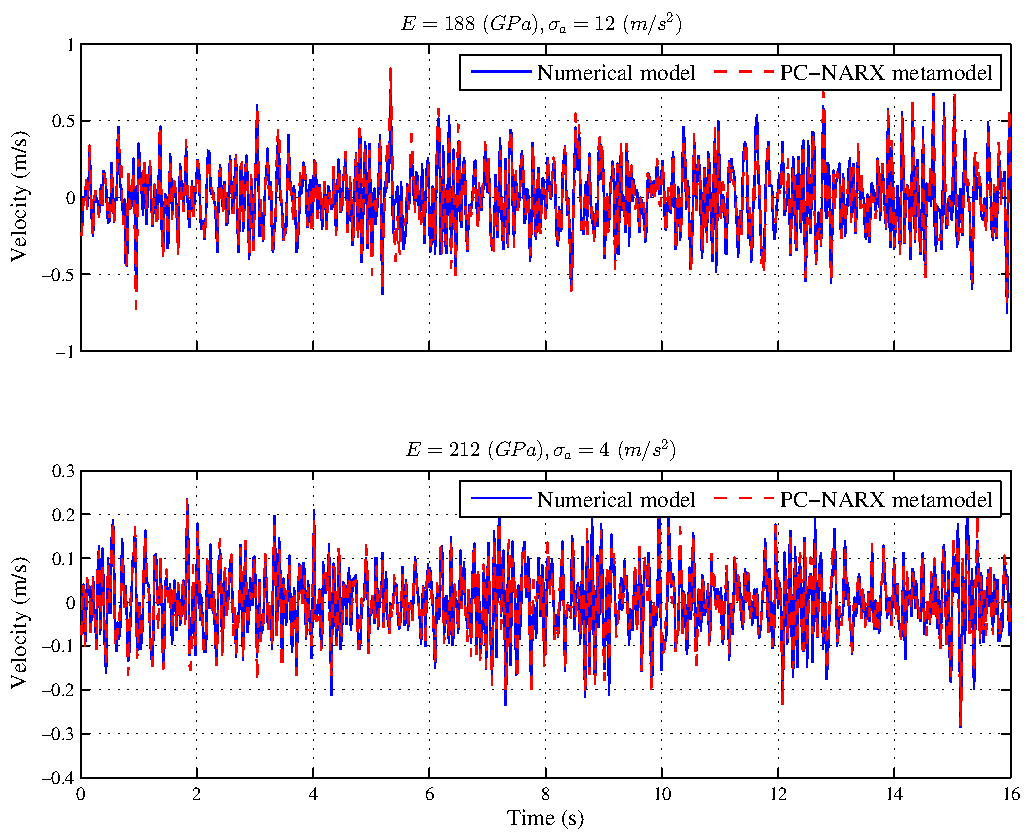
\includegraphics[width = 0.75\textwidth]{figs/SF_randexci_val.pdf}
\caption{Shear frame FE model PC-NARX metamodel validation: PC-NARX metamodel simulation contrasted to the simulations of the FE model for (a) $ E = 188$ GPa, $\sigma_a = 12$ (m/s$^2$), and (b) $ E = 212$ GPa ,$\sigma_a = 4$ (m/s$^2$). 
\label{fig:SF_validation}}
\end{center}
\end{figure}
% ================================================ 

% ================================================
\section{Conclusions}\label{sec:conclusions}
% ================================================
This work introduces a reduced order metamodel for nonlinear, dynamically evolving systems, based on NARX models and polynomial chaos expansion. The metamodel is identified through a multi-step procedure, which combines integer optimization and a backward selection scheme for the selection of the appropriate nonlinear regressors and the PC functional subspace and a nonlinear least squares optimization procedure for the estimation of the PC-NARX model based on the minimization of the simulation error criterion. In order to illustrate the workings of the method, the whole procedure was applied for the construction of a metamodel representation of two simple SDOF nonlinear systems and a multi-story shear frame FE model. The metamodels were estimated from simulated data obtained by the original finer details numerical models, with the properties of the systems assumed to be uncertain input variables following probability distributions with predefined characteristics. Overall, the study demonstrated the effectiveness and applicability of the proposed method for the estimation of stochastic, computationally inexpensive metamodels that are capable of accurate approximation of computationally costly numerical models.

%--------------------------------------------------------------------------------------------------
%                                   Bibliography
%--------------------------------------------------------------------------------------------------
\addcontentsline{toc}{section}{References}
\bibliographystyle{elsarticle-num}
\bibliography{PCNARX}

\end{document}








% Figure
% ================================================
%\begin{figure}[t!]
%\begin{center}
%\includegraphics[width = 1\textwidth]{figs/cubic_rss.pdf}
%\caption{PC-NARX metamodel prediction and simulation performance: (a) prediction and simulation for $y_7[t]$, and (b) standard deviation of the prediction error and simulation error residual sequences for all the simulation experiments. \label{fig:cubic_rss}}
%\end{center}
%\end{figure}
% ================================================


%Finally, the estimated PC-NARX metamodel is also successfully validated with respect to the assumptions on the residual sequences (see equation \ref{eq:assumptions}). More specifically, the uncrosscorrelatedness between the residual sequences $e_k^T (k=1,\ldots,K)$ may be illustrated through the almost diagonal covariance matrix $\mbox{cov}(\hat{\bld e}_{k_1}, \hat{\bld e}_{k_2})$ depicted in figure \ref{fig:cubic_validation}. The PC-NARX(8) based prediction and simulation values for one of the simulation experiments and the RMS values for the PE and SE residual sequences for all the simulation experiments are also depicted in Fig. \ref{fig:cubic_rss}.


% least squares method depending on the intended purpose of model use, prediction or simulation

% Finally, the estimated PC-NARX metamodel is validated through its usage for the simulation of 20 input variable vectors which where not used during the PC-NARX model structure and estimation procedure. The normalized squared sum of simulation errors obtained for both the estimation and validation sets are depicted in Fig. \ref{fig:cubic_validation}, and as it may be observed the levels of the errors are similar for both sets. 

% Also in this case, the metamodel should approximate the dynamic response of such a system in the discrete time domain.

% The selection of the regressors search space is based on the discretization of the ODE describing the hysteretic system by following a procedure similar with that described in the previous section for the system with cubic stiffness .



%For purposes of practicality, the infinite series of expansion of equation (\ref{eq:PCE}) must be truncated by selecting an appropriate functional subspace consisting of a finite number of terms $p$. In this way, the resulting PC-NARX model is fully parametrized in terms of a finite number of deterministic coefficients of projection $\theta_{i,j}$, while the complete PC-NARX identification problem consists of the subproblems of model parameter estimation and model structure selection, which are discussed in the following sections.


% The SE estimation method must be employed when a PC-NARX metamodel is intended to be used for simulation purposes, this means that in contrast to the PE case no information regarding the past values of the response are given. In this case, a metamodel that may replace the numerical model for additional simulations is sought. 

% According to the intended use of the metamodel the estimation of the parameter vector $\bth$ may be based upon the minimization of either the Prediction Error (PE) criterion or Simulation Error (SE) criterion. 



%%
% \beq 
% \bld{\vartheta}_i (\bxi) = \sum_{j=1}^{P} \theta_{i,j}\cdot \phi_{\bld{d}(j)}(\bxi) \quad \text{ with } P = 0,1,2,\ldots, P_{\text{max}} \label{eq:PCEmss}
% \eeq
%%
% and the proper maximum degree is selected based on the mean normalized expansion error
%%

%\beq 
%\text{MNE} = \frac{1}{K n_\vartheta} \sum_{i=1}^{n_\vartheta} \sum_{k=1}^K \left( \frac{ \mid \vartheta_{i_k}  - \sum_{j=1}^{P} \theta_{k,j}\cdot \phi_{\bld{d}(j)}(\bxi)\mid}{\mid \vartheta_{i_k} \mid }\right)  \label{eq:PCEerror}
%\eeq
%%

% The expansion parameters may be used as initial estimates for the final PC-NARX model which is refined through SE-based nonlinear optimization (Section \ref{sec:SEestimation}). 
%In order to illustrate this procedure consider an initial PC basis with total maximum degree $P = 2$ and $M = 3$ input random variables. The dimensionality of this basis will be equal to \cite{Blatman-Sudret2010}:
%%%
%$$ p = \frac{(M+P) !}{M! P !} = \frac{5!}{3!2!} = 10$$
%%%
%In order to represent all the functional subspaces included in this initial search space through a compact 10-bit binary vector, each multi-index vector ${\bld d}(j) \ (j =1,\ldots,10)$ may be represented by a single bit indicating the existence (1) or not (0) of the corresponding PC basis function in the specific model structure.




% Although the classical PC expansion approach has been proved to be a computationally efficient way for describing the uncertainty propagation \cite{Blatman-etal2010, Ghanem-Spanos2003} it cannot adequately handle time dependencies. In that case, the dynamics of the numerical model at each distinct time instant $t$ should be treated as a separate output and a PC expansion model should be identified, leading to a large number of parameters. In order to circumvent this difficulty a PC-ARX metamodeling method which is capable of approximating the numerical model dynamic behavior in an efficient way is introduced in this work. 

% PC expansion is based on Wiener's theory of homogeneous chaos [] and has gained particular attraction  offers a useful tool for the development of stochastic metamodels capable of representing the complete random responses of analytical models with uncertain input variables. This approach relies upon the approximation of the random response of an analytical large-scale model by a suitably defined finite-dimensional PC basis in order to create a low order metamodel. 

%Overall, this study aims at demonstrating the effectiveness and applicability of the proposed method for the estimation of stochastic metamodels of low order that are capable of accurate approximation of large-scale FE models.

% In order to improve the accuracy of the numerical analysis, the first one aims at developing mathematical models for new elements or at incorporating some features which make the existing elements able to solve new mechanical problems (i.e., in presence of high nonlinearities, time-dependent phenomena, fluid–structure interactions). In virtue of their feasibility, FE-based methods are powerful tools for assessing complex structural systems but require a very high computational cost to do it (especially for dynamic analyses). 

% We define simulation optimization as the latter case: repeated analysis of the simulation model with different values of design parameters, in an attempt to identify best simulated system performance. The design parameters of the real system are set to the ‘optimal’ parameter values determined by the simulation optimization exercise, rather than in an ad hoc manner based on qualitative insights gained from exercising the simulation model. We will use the following notation to represent the general simulation optimization problem, following Andradóttir (1998):

% where θ is the (possibly vector-valued) design parameter of the system being simulated, and the feasible region Θ∈Rd is the set of possible values of θ. The optimization model response function is represented by f(θ) which is usually the expected value (long-term average) of some simulated system performance measure Y as a function of the design parameter vector θ. That is, f(θ)=E(Y(θ)). The form of f is not known. Its value is estimated using n runs of the simulation model under the design scenario specified by ,

% Experimentation with computer simulation models of proposed or existing real structural systems is often used to make decisions on changes to the system design. Analysts exercise the simulation model because cost, time or other constraints prohibit experimentation with the real system. For the extensive experimentation required for optimization, the simulation models themselves may require excessive computation, and so simpler approximations are often constructed; models of the model, called metamodels ( [Kleijnen, 1975a], [Kleijnen, 1975b] and [Kleijnen, 1987]) or surrogate models (Yesilyurt and Patera, 1995). These metamodels are usually deterministic approximating functions for f that are inexpensive to compute. Running multiple replications of the simulation to produce  is expensive; running the metamodel once produces the deterministic value g(θ) which approximates f(θ) with low computational expense.

% Due to the fact that the computational burden of dynamic response simulation for time history loading is usually high, a metamodeling based method is sought. This method must be able to predict the dynamic response of the numerical model under study.

% The major issues in metamodeling include \cite{Barton-Meckesheimer2006}: {\em (i)} the choice of a functional form of the metamodel, {\em (ii)} the design of experiments, that is, the selection of a set of input variables values at which to observe the numerical model response by running the simulation model, {\em (iii)} fitting the metamodel to the simulation response using the experimental data, and {\em (iv)} the assessment of the adequacy of the fitted metamodel. 

% Considering that the structure under study may be approximated by an ARMA$(n_a,n_c)$ model of a-priori unknown AR/MA orders, $n_a$ and $n_c$ respectively, the ARMA model parameters will be also random variables represented by a deterministic mapping $\bth = \cal{M}(\bxi)$ which describes the relation between. 


% The applicability of the PC-NARX method will be assessed in this case study by assuming no-prior knowledge on the system dynamics and the type of nonlinearity. The nonlinear regressors search space consists of all regressors of the type . The estimated values are shown in Fig. and indicate the simulation experiment number ... as the one depicting the highest degree of nonlinearity among the 20 simulated responses. It is noted that for this simulation the cubic stiffness coefficient is equal to ... and the standard deviation of the random force excitation equal to (N).


%First, the total maximum degree $P$ is selected by examining the mean normalized error of the PC expansion for complete subspaces with $P = 0,\ldots,3$. As shown in Fig. \ref{fig:cubic_MSS_B}(a) $P=1$, that a multivariate basis consisting of the tensor products of Legendre polynomials of up to first degree, is adequate, while again a backward selection scheme [Fig. \ref{fig:cubic_MSS_B}(b)] may be used to drop one of the two non-constant basis function. 



%As it may be observed the despite the fact that the RMS of the PE values are below 10$^{-2}$ even for a PC-NARX model with 25 regressors, the simulation error is relatively high and gets only below 2 \% for this number of terms. This is due to the fact that the Bouc-Wen model may be considered as a piecewise linear model and so it may be approximated by linear models. 

% On the other hand, the accurate simulation of the oscillator is much more difficult since the nonlinear functions used for the PC-NARX model do not contain any absolute or signum functions so the approximation of the model necessities a high number of polynomial terms. For the same reason, the PC-NARX model parameters in this case show dependence on both the model characteristic $\beta$ and the level of excitation as clearly shown by the curve estimate of the parameter $\theta$ corresponding to the nonlinear regressor $y[t-3]^3$.

%The applicability of the PC-NARX method will be assessed in this case study by assuming no-prior knowledge on the system dynamics and the type of nonlinearity. The nonlinear PC-NARX regressors are selected based on the simulated responses which depicts the stronger nonlinearity according to the nonlinearity measure of Eq. (). The estimated values are shown in Fig. and indicate the simulation experiment number ... as the one depicting the highest degree of nonlinearity among the 20 simulated responses. It is noted that for this simulation the cubic stiffness coefficient is equal to ... and the standard deviation of the random force excitation equal to (N). 

